% !TEX root = ../dissertationOG.tex

\clearpage % clear the prior chapter's page
\chapter{Render-Guided Volumetric Morphing with Differentiable Physics}\label{CH4_PhysMorphGS}
% Packages used by this chapter: amsmath, graphicx, booktabs, array, tikz, algorithm + algpseudocode, natbib (\citep).
% The details of this chapter (constants, per-step updates, term formulas, selection rule, multi-body contact,
% implementation, measures, long tables) are in the appendix "Details of Chapter 4": docs/Chapter4_appendix.tex here,
% Sections/Appendix.tex in the dissertation build. Its labels (app:ch4*, ch4:sec_below_grid, ch4:sec_cleanup,
% ch4:sec_scene, ch4:tab_b1, ch4:tab_ablation, ch4:tab_methods, ...) are referenced from this chapter.
% Dissertation build: \usepackage{tikz} and \usetikzlibrary{positioning,arrows.meta,fit,calc} are loaded in the
% preamble of VanderbiltDissertationTemplate/dissertationOG.tex.
% Dissertation build: extra stretch for this chapter only (reset at its end), so that no line runs into the margin.
\setlength{\emergencystretch}{1.5em}

% ============================================================================
\section{Overview}
\label{ch4:sec_overview}
% ============================================================================

Chapter~\ref{CH3_SHAPEMORPHING} morphed one shape into another by optimizing per-particle control deformation
gradients in a differentiable MLS-MPM simulation. The control enters the material only as an internal stress, so the
morph conserves mass and momentum and can change topology. Its objective, however, was a mass loss on the background
grid, and its appearance was produced afterwards, when the particles were meshed and smoothed for rendering. Nothing a
viewer sees, neither the silhouette of the body nor the shading of its surface, took part in the control.

In this chapter we make the picture part of the control. We optimize the same kind of physical body so that it also
\emph{looks} like the target: differentiable rendering terms, evaluated on a surface built from the body's own particles,
steer the simulation through its controls, while the controls still enter the material only as a stress and as a
rigid-free offset of its surface. Three observations shape the method. A control that is scored while it is still pushing
can win a state that springs back once it lets go. A picture asks for changes at the scale of a pixel, below the MPM
cell, which a control acting only through the grid averages away over the many particles of a cell. And the pixels of a
rendered particle cloud are not those of the surface a viewer sees. Our pipeline answers each of them:
\begin{itemize}
  \item \textbf{Settled windows.} The body is optimized window by window, and each window is scored only after the
        controls have been released and the body has settled (Section~\ref{ch4:sec_method}).
  \item \textbf{Two controls on two scales.} A capped stress increment $\delta\mathbf{F}_c$ moves the bulk through the
        grid, as in Chapter~\ref{CH3_SHAPEMORPHING}; a rigid-free normal offset $u$ of the outer particle layer shapes the
        surface below the grid (Section~\ref{ch4:sec_controls}).
  \item \textbf{A volume-conserving body} whose particles carry the volume their motion makes
        (Section~\ref{ch4:sec_body}).
  \item \textbf{Render terms on the body's exterior}, the surface of the particles' own field, weighted against a
        transport-based physics objective (Section~\ref{ch4:sec_objective}).
\end{itemize}

One finding runs through the chapter, and we state it at the outset. In the pipeline as it stands, the render term earns
its effect mainly while the body is arriving: there it redirects material well beyond the run-to-run noise. Once the body
has arrived, its weight follows the vanishing physics gradient, and it only polishes the outline. The end is closer to the
exact target on every standard metric we read, but by fractions of a particle spacing. We measure each part of this
against a $\lambda=0$ twin, the same run with the render weight set to zero, and end the chapter with the step it points
to: keeping the render's authority after arrival, where it can decide what the physics objective cannot see. The
constants, the per-step updates and the longer tables are collected in Appendix~\ref{app:ch4}.

\begin{figure*}[t]
    \centering
    \resizebox{\textwidth}{!}{% Chapter 4 pipeline overview (TikZ; 2026-10-21 layout, after the user's sketch): the morph sequence on top, one
% window below it in three stages (simulation, exterior surface, rendering), the adjoint underneath, and the control
% update closing the loop on the left. The cleanup terms (spray pull, near band) are left out of the figure.
% Included by Chapter4.tex / Chapter4_ko.tex with
%   \resizebox{\textwidth}{!}{% Chapter 4 pipeline overview (TikZ; 2026-10-21 layout, after the user's sketch): the morph sequence on top, one
% window below it in three stages (simulation, exterior surface, rendering), the adjoint underneath, and the control
% update closing the loop on the left. The cleanup terms (spray pull, near band) are left out of the figure.
% Included by Chapter4.tex / Chapter4_ko.tex with
%   \resizebox{\textwidth}{!}{% Chapter 4 pipeline overview (TikZ; 2026-10-21 layout, after the user's sketch): the morph sequence on top, one
% window below it in three stages (simulation, exterior surface, rendering), the adjoint underneath, and the control
% update closing the loop on the left. The cleanup terms (spray pull, near band) are left out of the figure.
% Included by Chapter4.tex / Chapter4_ko.tex with
%   \resizebox{\textwidth}{!}{\input{figs/ch4/pipeline_overview.tikz}}
% Needs \usepackage{tikz,graphicx,amsmath} and \usetikzlibrary{arrows.meta}, loaded once outside any group.
% Font sizes are fixed in pt (as the SVG's px: 18 px = 6.4 pt), so the class's size option does not change the layout.
% The same diagram, hand-written, is pipeline_overview.svg in this folder: keep the two in sync.
% Coordinates in cm: 1 cm = 80 px of the SVG, x = x_svg / 80, y = 10 - y_svg / 80.
% Tiles: figs/ch4/overview_tiles/tile0-4.jpg (bunny 300k, tag freeze-2026-10-15, seed 97, full arm, studio look,
% t = 0, 0.5, 1, 2 s and the last kept frame, 15.7 s). The previous, detailed diagram is kept in
% src_pipeline_overview/previous_detailed/.
\begin{tikzpicture}[
  font=\fontsize{6.2}{8.9}\selectfont,
  flow/.style={-{Latex[length=2mm]}, line width=0.6pt},
  stage/.style={draw, line width=0.6pt},
  body/.style={anchor=north west, align=left, inner sep=0pt, text width=#1,
    execute at begin node={\hyphenpenalty=10000\exhyphenpenalty=10000}},
  title/.style={anchor=base west, inner sep=0pt, font=\fontsize{6.8}{8}\selectfont},
  small/.style={font=\fontsize{5.6}{6.8}\selectfont},
  slant/.style={font=\fontsize{6}{7}\selectfont\itshape},
]
% ---------------------------------------------------------------- the morph sequence
\node[small] at (11.0,9.75) {E\,N\,T\,I\,R\,E\ \ M\,O\,R\,P\,H\,I\,N\,G\ \ S\,E\,Q\,U\,E\,N\,C\,E};
\draw[flow] (5.4,9.575) -- (16.6,9.575);
\foreach \i/\x in {0/5.4, 1/7.55, 2/9.7, 3/11.85, 4/14.725} {
  \begin{scope}
    \clip[rounded corners=0.1cm] (\x,7.5) rectangle ++(1.875,1.875);
    \node[inner sep=0pt, anchor=south west] at (\x,7.5)
      {\includegraphics[width=1.875cm]{figs/ch4/overview_tiles/tile\i.jpg}};
  \end{scope}
}
\node at (14.225,8.44) {$\cdots$};
\foreach \x/\t in {6.3375/{Initial ($t = 0$)}, 8.4875/{0.5\,s}, 10.6375/{1\,s}, 12.7875/{2\,s}, 15.6625/{Final (15.7\,s)}}
  \node[small, anchor=base] at (\x,7.2) {\t};

% ---------------------------------------------------------------- one window
\fill[black!11] (5.25,7.05) -- (16.75,7.05) -- (15.25,6.025) -- (6.75,6.025) -- cycle;
\node[slant, anchor=base] at (11.0,6.65)
  {one window $k$ = $2T$ steps (1/6\,s), optimised over its controls,};
\node[slant, anchor=base] at (11.0,6.325)
  {then committed (plastic assimilation of $\mathbf{F}_p$; accept or reject; stop rule) $\rightarrow$ window $k+1$};

% ---------------------------------------------------------------- the three stages
\node[title] at (3.375,5.725) {(1) Differentiable MLS-MPM};
\node[title] at (8.8125,5.725) {(2) Exterior Surface};
\node[title] at (13.75,5.725) {(3) Differentiable Rendering};
\draw[stage] (3.375,5.6) rectangle (8.25,2.7);
\draw[stage] (8.8125,5.6) rectangle (13.1875,2.7);
\draw[stage] (13.75,5.6) rectangle (18.625,2.7);
\node[body=4.55cm] at (3.55,5.45) {%
  \textit{Forward simulation ($2T$ steps)}\\
  - driven half: $\delta\mathbf{F}_c$ and $u$ act\\
  - released half: controls set to zero\\
  - P2G\,/\,grid\,/\,G2P\\
  - outer-layer relaxation\\[3pt]
  \textit{Physics loss on the released end state}\\
  - Sinkhorn transport to the target\\
  - proximity, end drift, released motion};
\node[body=4.0cm] at (8.9875,5.45) {%
  \textit{Surface from the particles}\\
  - Zhu--Bridson field of the particles\\
  - exterior discs on its zero level\\
  - normals from the field\\[3pt]
  \textit{Differentiable}\\
  - the discs move with the particles,\\
  \hphantom{- }so render gradients reach them};
\node[body=4.55cm] at (13.925,5.45) {%
  \textit{Render}\\
  - soft splats of the discs\\
  - 18 orthographic views\\
  - silhouette and Lambert shading\\[3pt]
  \textit{Render loss}\\
  - $\mathcal{L}_{\mathrm{sil}} + \mathcal{L}_{\mathrm{shade}}$ against the pictures\\
  \hphantom{- }of the target (the same 18 views)};

% ---------------------------------------------------------------- input and stage arrows
\node[align=center, font=\fontsize{6.8}{8.4}\selectfont] at (1.5,3.95)
  {Input\\[1pt] $\delta\mathbf{F}_c,\ u$\\[1pt]
   {\fontsize{5.6}{6.8}\selectfont (controls,}\\ {\fontsize{5.6}{6.8}\selectfont iteration $i$)}};
\draw[flow] (2.375,3.925) -- (3.375,3.925);
\draw[flow] (8.25,3.925) -- (8.8125,3.925);
\draw[flow] (13.1875,3.925) -- (13.75,3.925);

% ---------------------------------------------------------------- gradients and the adjoint
\draw[flow] (5.8125,2.7) -- (5.8125,1.825);
\node[anchor=west] at (6.0,2.2) {$\nabla\mathcal{L}_{\mathrm{phys}}$};
\draw[flow] (16.1875,2.7) -- (16.1875,1.825);
\node[anchor=west] at (16.375,2.2) {$\nabla\mathcal{L}_{\mathrm{render}}$};
\draw[stage] (3.375,1.825) rectangle (18.625,0.45);
\node[align=center, font=\fontsize{6}{8}\selectfont] at (11.0,1.1375) {%
  {\fontsize{6.8}{8}\selectfont Adjoint through the $2T$ steps (reverse mode of the same MLS-MPM)}\\[2pt]
  {\fontsize{7.8}{9.4}\selectfont $\mathcal{L}_{\mathrm{total}} = \mathcal{L}_{\mathrm{phys}} + \lambda\,\mathcal{L}_{\mathrm{render}}$}\\[2pt]
  PCGrad drops the part of $\nabla\mathcal{L}_{\mathrm{render}}$ that opposes $\nabla\mathcal{L}_{\mathrm{phys}}$;\quad
  $\lambda\,\lVert\nabla\mathcal{L}_{\mathrm{render}}\rVert = \tfrac12\lVert\nabla\mathcal{L}_{\mathrm{phys}}\rVert$};

% ---------------------------------------------------------------- control update
\draw[stage] (0.25,2.075) rectangle (2.5,0.2);
\node[align=center, font=\fontsize{5.7}{7.8}\selectfont] at (1.375,1.1375) {%
  {\fontsize{6.8}{8}\selectfont\itshape Control update}\\[2pt]
  Adam step with\\ line search;\\ $\delta\mathbf{F}_c$ capped;\\ $u$ free of\\ rigid modes};
\draw[flow] (3.375,1.1375) -- (2.5,1.1375);
\node[align=center, font=\fontsize{5.3}{6.4}\selectfont] at (2.9375,1.5) {inject\\ $\nabla\mathcal{L}_{\mathrm{total}}$};
\draw[flow] (1.375,2.075) -- (1.375,3.15);
\end{tikzpicture}
}
% Needs \usepackage{tikz,graphicx,amsmath} and \usetikzlibrary{arrows.meta}, loaded once outside any group.
% Font sizes are fixed in pt (as the SVG's px: 18 px = 6.4 pt), so the class's size option does not change the layout.
% The same diagram, hand-written, is pipeline_overview.svg in this folder: keep the two in sync.
% Coordinates in cm: 1 cm = 80 px of the SVG, x = x_svg / 80, y = 10 - y_svg / 80.
% Tiles: figs/ch4/overview_tiles/tile0-4.jpg (bunny 300k, tag freeze-2026-10-15, seed 97, full arm, studio look,
% t = 0, 0.5, 1, 2 s and the last kept frame, 15.7 s). The previous, detailed diagram is kept in
% src_pipeline_overview/previous_detailed/.
\begin{tikzpicture}[
  font=\fontsize{6.2}{8.9}\selectfont,
  flow/.style={-{Latex[length=2mm]}, line width=0.6pt},
  stage/.style={draw, line width=0.6pt},
  body/.style={anchor=north west, align=left, inner sep=0pt, text width=#1,
    execute at begin node={\hyphenpenalty=10000\exhyphenpenalty=10000}},
  title/.style={anchor=base west, inner sep=0pt, font=\fontsize{6.8}{8}\selectfont},
  small/.style={font=\fontsize{5.6}{6.8}\selectfont},
  slant/.style={font=\fontsize{6}{7}\selectfont\itshape},
]
% ---------------------------------------------------------------- the morph sequence
\node[small] at (11.0,9.75) {E\,N\,T\,I\,R\,E\ \ M\,O\,R\,P\,H\,I\,N\,G\ \ S\,E\,Q\,U\,E\,N\,C\,E};
\draw[flow] (5.4,9.575) -- (16.6,9.575);
\foreach \i/\x in {0/5.4, 1/7.55, 2/9.7, 3/11.85, 4/14.725} {
  \begin{scope}
    \clip[rounded corners=0.1cm] (\x,7.5) rectangle ++(1.875,1.875);
    \node[inner sep=0pt, anchor=south west] at (\x,7.5)
      {\includegraphics[width=1.875cm]{figs/ch4/overview_tiles/tile\i.jpg}};
  \end{scope}
}
\node at (14.225,8.44) {$\cdots$};
\foreach \x/\t in {6.3375/{Initial ($t = 0$)}, 8.4875/{0.5\,s}, 10.6375/{1\,s}, 12.7875/{2\,s}, 15.6625/{Final (15.7\,s)}}
  \node[small, anchor=base] at (\x,7.2) {\t};

% ---------------------------------------------------------------- one window
\fill[black!11] (5.25,7.05) -- (16.75,7.05) -- (15.25,6.025) -- (6.75,6.025) -- cycle;
\node[slant, anchor=base] at (11.0,6.65)
  {one window $k$ = $2T$ steps (1/6\,s), optimised over its controls,};
\node[slant, anchor=base] at (11.0,6.325)
  {then committed (plastic assimilation of $\mathbf{F}_p$; accept or reject; stop rule) $\rightarrow$ window $k+1$};

% ---------------------------------------------------------------- the three stages
\node[title] at (3.375,5.725) {(1) Differentiable MLS-MPM};
\node[title] at (8.8125,5.725) {(2) Exterior Surface};
\node[title] at (13.75,5.725) {(3) Differentiable Rendering};
\draw[stage] (3.375,5.6) rectangle (8.25,2.7);
\draw[stage] (8.8125,5.6) rectangle (13.1875,2.7);
\draw[stage] (13.75,5.6) rectangle (18.625,2.7);
\node[body=4.55cm] at (3.55,5.45) {%
  \textit{Forward simulation ($2T$ steps)}\\
  - driven half: $\delta\mathbf{F}_c$ and $u$ act\\
  - released half: controls set to zero\\
  - P2G\,/\,grid\,/\,G2P\\
  - outer-layer relaxation\\[3pt]
  \textit{Physics loss on the released end state}\\
  - Sinkhorn transport to the target\\
  - proximity, end drift, released motion};
\node[body=4.0cm] at (8.9875,5.45) {%
  \textit{Surface from the particles}\\
  - Zhu--Bridson field of the particles\\
  - exterior discs on its zero level\\
  - normals from the field\\[3pt]
  \textit{Differentiable}\\
  - the discs move with the particles,\\
  \hphantom{- }so render gradients reach them};
\node[body=4.55cm] at (13.925,5.45) {%
  \textit{Render}\\
  - soft splats of the discs\\
  - 18 orthographic views\\
  - silhouette and Lambert shading\\[3pt]
  \textit{Render loss}\\
  - $\mathcal{L}_{\mathrm{sil}} + \mathcal{L}_{\mathrm{shade}}$ against the pictures\\
  \hphantom{- }of the target (the same 18 views)};

% ---------------------------------------------------------------- input and stage arrows
\node[align=center, font=\fontsize{6.8}{8.4}\selectfont] at (1.5,3.95)
  {Input\\[1pt] $\delta\mathbf{F}_c,\ u$\\[1pt]
   {\fontsize{5.6}{6.8}\selectfont (controls,}\\ {\fontsize{5.6}{6.8}\selectfont iteration $i$)}};
\draw[flow] (2.375,3.925) -- (3.375,3.925);
\draw[flow] (8.25,3.925) -- (8.8125,3.925);
\draw[flow] (13.1875,3.925) -- (13.75,3.925);

% ---------------------------------------------------------------- gradients and the adjoint
\draw[flow] (5.8125,2.7) -- (5.8125,1.825);
\node[anchor=west] at (6.0,2.2) {$\nabla\mathcal{L}_{\mathrm{phys}}$};
\draw[flow] (16.1875,2.7) -- (16.1875,1.825);
\node[anchor=west] at (16.375,2.2) {$\nabla\mathcal{L}_{\mathrm{render}}$};
\draw[stage] (3.375,1.825) rectangle (18.625,0.45);
\node[align=center, font=\fontsize{6}{8}\selectfont] at (11.0,1.1375) {%
  {\fontsize{6.8}{8}\selectfont Adjoint through the $2T$ steps (reverse mode of the same MLS-MPM)}\\[2pt]
  {\fontsize{7.8}{9.4}\selectfont $\mathcal{L}_{\mathrm{total}} = \mathcal{L}_{\mathrm{phys}} + \lambda\,\mathcal{L}_{\mathrm{render}}$}\\[2pt]
  PCGrad drops the part of $\nabla\mathcal{L}_{\mathrm{render}}$ that opposes $\nabla\mathcal{L}_{\mathrm{phys}}$;\quad
  $\lambda\,\lVert\nabla\mathcal{L}_{\mathrm{render}}\rVert = \tfrac12\lVert\nabla\mathcal{L}_{\mathrm{phys}}\rVert$};

% ---------------------------------------------------------------- control update
\draw[stage] (0.25,2.075) rectangle (2.5,0.2);
\node[align=center, font=\fontsize{5.7}{7.8}\selectfont] at (1.375,1.1375) {%
  {\fontsize{6.8}{8}\selectfont\itshape Control update}\\[2pt]
  Adam step with\\ line search;\\ $\delta\mathbf{F}_c$ capped;\\ $u$ free of\\ rigid modes};
\draw[flow] (3.375,1.1375) -- (2.5,1.1375);
\node[align=center, font=\fontsize{5.3}{6.4}\selectfont] at (2.9375,1.5) {inject\\ $\nabla\mathcal{L}_{\mathrm{total}}$};
\draw[flow] (1.375,2.075) -- (1.375,3.15);
\end{tikzpicture}
}
% Needs \usepackage{tikz,graphicx,amsmath} and \usetikzlibrary{arrows.meta}, loaded once outside any group.
% Font sizes are fixed in pt (as the SVG's px: 18 px = 6.4 pt), so the class's size option does not change the layout.
% The same diagram, hand-written, is pipeline_overview.svg in this folder: keep the two in sync.
% Coordinates in cm: 1 cm = 80 px of the SVG, x = x_svg / 80, y = 10 - y_svg / 80.
% Tiles: figs/ch4/overview_tiles/tile0-4.jpg (bunny 300k, tag freeze-2026-10-15, seed 97, full arm, studio look,
% t = 0, 0.5, 1, 2 s and the last kept frame, 15.7 s). The previous, detailed diagram is kept in
% src_pipeline_overview/previous_detailed/.
\begin{tikzpicture}[
  font=\fontsize{6.2}{8.9}\selectfont,
  flow/.style={-{Latex[length=2mm]}, line width=0.6pt},
  stage/.style={draw, line width=0.6pt},
  body/.style={anchor=north west, align=left, inner sep=0pt, text width=#1,
    execute at begin node={\hyphenpenalty=10000\exhyphenpenalty=10000}},
  title/.style={anchor=base west, inner sep=0pt, font=\fontsize{6.8}{8}\selectfont},
  small/.style={font=\fontsize{5.6}{6.8}\selectfont},
  slant/.style={font=\fontsize{6}{7}\selectfont\itshape},
]
% ---------------------------------------------------------------- the morph sequence
\node[small] at (11.0,9.75) {E\,N\,T\,I\,R\,E\ \ M\,O\,R\,P\,H\,I\,N\,G\ \ S\,E\,Q\,U\,E\,N\,C\,E};
\draw[flow] (5.4,9.575) -- (16.6,9.575);
\foreach \i/\x in {0/5.4, 1/7.55, 2/9.7, 3/11.85, 4/14.725} {
  \begin{scope}
    \clip[rounded corners=0.1cm] (\x,7.5) rectangle ++(1.875,1.875);
    \node[inner sep=0pt, anchor=south west] at (\x,7.5)
      {\includegraphics[width=1.875cm]{figs/ch4/overview_tiles/tile\i.jpg}};
  \end{scope}
}
\node at (14.225,8.44) {$\cdots$};
\foreach \x/\t in {6.3375/{Initial ($t = 0$)}, 8.4875/{0.5\,s}, 10.6375/{1\,s}, 12.7875/{2\,s}, 15.6625/{Final (15.7\,s)}}
  \node[small, anchor=base] at (\x,7.2) {\t};

% ---------------------------------------------------------------- one window
\fill[black!11] (5.25,7.05) -- (16.75,7.05) -- (15.25,6.025) -- (6.75,6.025) -- cycle;
\node[slant, anchor=base] at (11.0,6.65)
  {one window $k$ = $2T$ steps (1/6\,s), optimised over its controls,};
\node[slant, anchor=base] at (11.0,6.325)
  {then committed (plastic assimilation of $\mathbf{F}_p$; accept or reject; stop rule) $\rightarrow$ window $k+1$};

% ---------------------------------------------------------------- the three stages
\node[title] at (3.375,5.725) {(1) Differentiable MLS-MPM};
\node[title] at (8.8125,5.725) {(2) Exterior Surface};
\node[title] at (13.75,5.725) {(3) Differentiable Rendering};
\draw[stage] (3.375,5.6) rectangle (8.25,2.7);
\draw[stage] (8.8125,5.6) rectangle (13.1875,2.7);
\draw[stage] (13.75,5.6) rectangle (18.625,2.7);
\node[body=4.55cm] at (3.55,5.45) {%
  \textit{Forward simulation ($2T$ steps)}\\
  - driven half: $\delta\mathbf{F}_c$ and $u$ act\\
  - released half: controls set to zero\\
  - P2G\,/\,grid\,/\,G2P\\
  - outer-layer relaxation\\[3pt]
  \textit{Physics loss on the released end state}\\
  - Sinkhorn transport to the target\\
  - proximity, end drift, released motion};
\node[body=4.0cm] at (8.9875,5.45) {%
  \textit{Surface from the particles}\\
  - Zhu--Bridson field of the particles\\
  - exterior discs on its zero level\\
  - normals from the field\\[3pt]
  \textit{Differentiable}\\
  - the discs move with the particles,\\
  \hphantom{- }so render gradients reach them};
\node[body=4.55cm] at (13.925,5.45) {%
  \textit{Render}\\
  - soft splats of the discs\\
  - 18 orthographic views\\
  - silhouette and Lambert shading\\[3pt]
  \textit{Render loss}\\
  - $\mathcal{L}_{\mathrm{sil}} + \mathcal{L}_{\mathrm{shade}}$ against the pictures\\
  \hphantom{- }of the target (the same 18 views)};

% ---------------------------------------------------------------- input and stage arrows
\node[align=center, font=\fontsize{6.8}{8.4}\selectfont] at (1.5,3.95)
  {Input\\[1pt] $\delta\mathbf{F}_c,\ u$\\[1pt]
   {\fontsize{5.6}{6.8}\selectfont (controls,}\\ {\fontsize{5.6}{6.8}\selectfont iteration $i$)}};
\draw[flow] (2.375,3.925) -- (3.375,3.925);
\draw[flow] (8.25,3.925) -- (8.8125,3.925);
\draw[flow] (13.1875,3.925) -- (13.75,3.925);

% ---------------------------------------------------------------- gradients and the adjoint
\draw[flow] (5.8125,2.7) -- (5.8125,1.825);
\node[anchor=west] at (6.0,2.2) {$\nabla\mathcal{L}_{\mathrm{phys}}$};
\draw[flow] (16.1875,2.7) -- (16.1875,1.825);
\node[anchor=west] at (16.375,2.2) {$\nabla\mathcal{L}_{\mathrm{render}}$};
\draw[stage] (3.375,1.825) rectangle (18.625,0.45);
\node[align=center, font=\fontsize{6}{8}\selectfont] at (11.0,1.1375) {%
  {\fontsize{6.8}{8}\selectfont Adjoint through the $2T$ steps (reverse mode of the same MLS-MPM)}\\[2pt]
  {\fontsize{7.8}{9.4}\selectfont $\mathcal{L}_{\mathrm{total}} = \mathcal{L}_{\mathrm{phys}} + \lambda\,\mathcal{L}_{\mathrm{render}}$}\\[2pt]
  PCGrad drops the part of $\nabla\mathcal{L}_{\mathrm{render}}$ that opposes $\nabla\mathcal{L}_{\mathrm{phys}}$;\quad
  $\lambda\,\lVert\nabla\mathcal{L}_{\mathrm{render}}\rVert = \tfrac12\lVert\nabla\mathcal{L}_{\mathrm{phys}}\rVert$};

% ---------------------------------------------------------------- control update
\draw[stage] (0.25,2.075) rectangle (2.5,0.2);
\node[align=center, font=\fontsize{5.7}{7.8}\selectfont] at (1.375,1.1375) {%
  {\fontsize{6.8}{8}\selectfont\itshape Control update}\\[2pt]
  Adam step with\\ line search;\\ $\delta\mathbf{F}_c$ capped;\\ $u$ free of\\ rigid modes};
\draw[flow] (3.375,1.1375) -- (2.5,1.1375);
\node[align=center, font=\fontsize{5.3}{6.4}\selectfont] at (2.9375,1.5) {inject\\ $\nabla\mathcal{L}_{\mathrm{total}}$};
\draw[flow] (1.375,2.075) -- (1.375,3.15);
\end{tikzpicture}
}
    \caption{Pipeline overview. \textmd{Each window simulates driven and released steps, scores the released end by the
    physics terms and by the silhouette and shading of the body's exterior from 18 views, and updates both controls
    through one adjoint (the two cleanup terms of Appendix~\ref{ch4:sec_cleanup} are omitted).}}
    \label{fig:overview}
\end{figure*}

% ============================================================================
\section{The Simulated Body}
\label{ch4:sec_body}
% ============================================================================

We build on the MLS-MPM simulator of Chapter~\ref{CH3_SHAPEMORPHING}, with cubic B-spline weights, APIC
transfers~\citep{jiang2016material} and the fixed corotated elastic response. The source (a sphere) and the target mesh
are each sampled into $N$ particles of equal mass, with the source rescaled to the target's volume, and we call
$a=(V/N)^{1/3}$, the edge of the volume per particle, the \emph{sampling pitch}. The MPM cell is set by the shape, not by
$N$, so at 300k particles a cell holds about 183 of them. This is why so much of what a picture asks for lies below the
grid. In a driven step the control enters the elastic deformation,
\begin{equation}
\label{eq:control_F}
\mathbf{F}^{\mathrm{E}}_p=\big(\mathbf{F}_p+\delta\mathbf{F}_{c,p}\big)\big(\mathbf{F}^{\mathrm{P}}_p\big)^{-1},
\qquad
\boldsymbol{\tau}_p=\mathbf{P}\big(\mathbf{F}^{\mathrm{E}}_p\big)\,\mathbf{F}^{\mathrm{E}\top}_p ,
\end{equation}
and the Kirchhoff stress $\boldsymbol{\tau}_p$ enters the particle-to-grid transfer as in Chapter~\ref{CH3_SHAPEMORPHING}.

Three additions keep the body's volume and its surface in order (Appendix~\ref{app:ch4_body}). Each particle carries the
volume its motion makes, so that the smoothing of the deformation gradient used in Chapter~\ref{CH3_SHAPEMORPHING} no
longer lets thin parts in transit dilate. At every commit, a plastic assimilation turns half of the elastic stretch,
volume included, into rest shape, so the end of a morph is the body's own rest. And three position updates act below the
grid: a minimum spacing that pushes too-close particles apart with equal and opposite pushes, a rigid-free relaxation of
the outer layer toward the target's relief, and bonds that keep detached fragments with their neighbours.

% ============================================================================
\section{Stress and Surface Controls}
\label{ch4:sec_controls}
% ============================================================================

As in Chapter~\ref{CH3_SHAPEMORPHING}, we drive the morph through the material's internal deformation rather than
through prescribed trajectories or external forces. A rendering term, however, asks for changes at two scales: the bulk
of the body has to travel to the target, which the grid can carry, and its surface has to take the target's outline and
relief, much of which lies below one MPM cell. We therefore give the optimizer two controls.

\subsection{The Stress Increment}
In each of the $T$ driven steps every particle has a $3\times3$ increment $\delta\mathbf{F}^{n}_{c,p}$, the control
deformation gradient of Chapter~\ref{CH3_SHAPEMORPHING}, capped per particle and step. It enters only through
Eq.~\eqref{eq:control_F}. Because the stress enters the grid as $\boldsymbol{\tau}_p(\mathbf{x}_i-\mathbf{x}_p)$ and the
B-spline weights satisfy $\sum_i w_{ip}(\mathbf{x}_i-\mathbf{x}_p)=\mathbf{0}$, the control cannot change the total linear
momentum, and since $\boldsymbol{\tau}_p$ is symmetric, APIC keeps the angular momentum as well~\citep{jiang2016material}.
One might instead drive the body with optimized external forces; Section~\ref{ch4:sec_force} makes that replacement and
measures what changes.

\subsection{The Layer Offset}
Every outer-layer particle has one scalar $u_p$ per window, a displacement along its normal applied in $T$ equal parts
over the driven steps:
\begin{equation}
\label{ch4:eq_u}
\mathbf{x}_p\leftarrow\mathbf{x}_p+\Big(\tfrac{1}{T}\,g_p\,u_p+s'_p\Big)\mathbf{n}_p ,
\end{equation}
where $s'_p$ is the relaxation step of Appendix~\ref{ch4:sec_below_grid} and $g_p\in\{0,1\}$ a gate. Its adjoint is the
identity times the physics' response, so the render gradient reaches it without the grid's low-pass. Three rules keep it a
surface control rather than a hand edit. It acts only on particles whose remaining transport is within one MPM cell, so it
shapes an arriving surface rather than carrying material. It is projected free of the six rigid modes of the layer after
every step of the optimizer, so it moves the body neither along nor about any axis. And it is bounded by one spacing per
window. Whether the physics holds what $u$ moves is decided by the released half of the window, in which $u$ does not act.

% ============================================================================
\section{Objective}
\label{ch4:sec_objective}
% ============================================================================

The objective has eight terms in three groups,
\begin{equation}
\label{ch4:eq_objective}
\mathcal{L}=\underbrace{\sigma\big(\mathcal{L}_{\mathrm{OT}}+\mathcal{L}_{\mathrm{prox}}+\mathcal{L}_{\mathrm{drift}}\big)
 +\mathcal{L}_{\mathrm{rel}}}_{\mathcal{L}_{\mathrm{phys}}}
 \;+\;\underbrace{0.2\,\big(\mathcal{L}_{\mathrm{spray}}+\mathcal{L}_{\mathrm{near}}\big)}_{\mathcal{L}_{\mathrm{clean}}}
 \;+\;\lambda\underbrace{\big(\mathcal{L}_{\mathrm{sil}}+\mathcal{L}_{\mathrm{shade}}\big)}_{\mathcal{L}_{\mathrm{render}}} ,
\end{equation}
whose formulas are given in Appendix~\ref{app:ch4_terms}. We kept a term only if switching it off changed a measured
quantity on a 19-mesh gallery and at 300k particles. The geometry and settling terms carry no weight of their own: $\sigma$
is one constant, measured once at the source, that gives the geometry energy the gradient norm of a log-mass grid loss of
the kind used in Chapter~\ref{CH3_SHAPEMORPHING}. There is no regularizer of the control or of the volume.

\subsection{What the Physics Terms Ask}
The \emph{transport} $\mathcal{L}_{\mathrm{OT}}$ is the debiased Sinkhorn divergence~\citep{feydy2019sinkhorn} between the
body's mass and the target's on a loss grid. The choice matters for the morph. The nodal mass residual of
Chapter~\ref{CH3_SHAPEMORPHING} has its gradient only where the density jumps at the surface, so it cannot see a filled
region that is merely in the wrong place; the transport's gradient is a transport field over the whole body, and it is
indifferent to topology. Because the transport blurs positions within a loss cell, the \emph{surface proximity}
$\mathcal{L}_{\mathrm{prox}}$ asks, at every outer point of the target, whether body material is there. Two settling terms
ask for an end at rest: the \emph{end drift} $\mathcal{L}_{\mathrm{drift}}$ charges the velocity left at the released end,
and the \emph{released motion} $\mathcal{L}_{\mathrm{rel}}$ charges all motion during the released half; without the
latter, runs stop while the body is still moving. Two local \emph{cleanup} terms with fixed weights,
Eqs.~\eqref{ch4:eq_spray} and~\eqref{ch4:eq_near}, pull isolated particles and particles just off the target surface back
toward it, where the transport cannot resolve them.

\subsection{Render Terms on the Exterior}
\label{ch4:sec_exterior}
The render terms read the surface of the body, not its particle cloud. The body's \emph{exterior} is the zero set of Zhu
and Bridson's field~\citep{10.1145/1073204.1073298} of the particles, covered by surface discs that follow the particles. The
\emph{silhouette} term compares the discs' coverage in 18 orthographic views with the target's, penalizing missing
coverage inside the target more than excess outside it; the \emph{shading} term compares headlight-lit images of the
discs. The target pictures are drawn by the same operator from the exterior of the target sample, averaged over eight
independent samples of the mesh so that the reference carries no single sample's noise (Appendix~\ref{app:ch4_render}).
Reading the render terms on the exterior rather than on the particle cloud is what makes them act on the surface a viewer
sees: read on the cloud, they improve the cloud's own silhouette and leave the displayed surface where the twin has it
(Section~\ref{ch4:sec_ablation}). The images in this chapter draw the same exterior with surface discs in a studio look;
every image is a committed simulated state.

% ============================================================================
\section{Morphing Method}
\label{ch4:sec_method}
% ============================================================================

Given the body, its controls and the objective, the morph is an optimization over a sequence of short simulation
networks, as in Chapter~\ref{CH3_SHAPEMORPHING}. Here each network is a settled window, and a window is committed only
after the body has been released and scored.

\subsection{Settled Windows}
A window simulates $T$ driven steps with the controls, then $T$ released steps with the controls at zero while the
physics keeps running. Every term of the objective is evaluated on the released end state and the released velocities.
Rebound, ringing and anything else that the control holds only while it pushes therefore cost the control directly. The
optimizer runs a fixed number of iterations per window; the window is then committed, and the next one starts from the
committed state (Algorithm~\ref{ch4:alg_window}).

\subsection{Gradients and the Render Weight}
\label{ch4:sec_lambda}
The physics, cleanup and render terms are differentiated separately through the same $2T$-step adjoint back to every
$\delta\mathbf{F}^n_{c}$ and to $u$. Let $\mathbf{g}_p$ be the gradient of the physics core and $\mathbf{g}_r$ that of the
render term. The render gradient loses its component against the physics gradient when the two
conflict~\citep{yu2020pcgrad},
\begin{equation}
\tilde{\mathbf{g}}_r=\mathbf{g}_r-\frac{\min(0,\langle\mathbf{g}_p,\mathbf{g}_r\rangle)}{\lVert\mathbf{g}_p\rVert^{2}}\,\mathbf{g}_p ,
\end{equation}
and the render weight is set at each window's first gradient by
\begin{equation}
\label{ch4:eq_lambda}
\lambda\,\lVert\tilde{\mathbf{g}}_r\rVert=\tfrac12\,\lVert\mathbf{g}_p\rVert ,
\end{equation}
so that the render term holds one third of the first gradient in every window. The step direction is
$\mathbf{g}=\mathbf{g}_p+\lambda\tilde{\mathbf{g}}_r+\mathbf{g}_{\mathrm{clean}}$.

This rule keeps the render's \emph{share} of a step constant, but not its \emph{authority}. While the body arrives, the
physics gradient falls by orders of magnitude, and $\lambda$ falls with it. The render term therefore acts strongly while
the body is on its way and only weakly once it has arrived, a consequence we measure in
Section~\ref{ch4:sec_render_effect} and take up again in Section~\ref{ch4:sec_costs}.

\subsection{Step, Commit and Stop}
The step is Adam's~\citep{kingma2014adam} with a backtracking line search, as in
Chapter~\ref{CH3_SHAPEMORPHING}; after each trial $\delta\mathbf{F}_c$ is capped and $u$ is bounded and made rigid-free.
The moments of $u$ carry from one window to the next, so that its first step in a window does not reverse the last one.
A window's result is committed together with the plastic assimilation, rejected if it raises the objective markedly, and
the run stops when the objective no longer improves (Appendix~\ref{app:ch4_method}).

\begin{algorithm}[t]
  \caption{Settled-window morph}\label{ch4:alg_window}
  \begin{algorithmic}[1]
    \Require source and target samples, $T$ driven and $T$ released steps, $i_{\max}$ iterations per window
    \State $\mathbf{s}\gets$ the source body at rest;\ $\delta\mathbf{F}^{\mathrm{prev}}_c\gets\mathbf{0}$
    \While{the stop rule has not fired}
      \State $\delta\mathbf{F}_c\gets\tfrac12\delta\mathbf{F}^{\mathrm{prev}}_c$ if that beats zero, else $\mathbf{0}$;\ $u\gets 0$
      \For{$i=1,\dots,i_{\max}$}
        \State simulate $T$ driven steps ($\delta\mathbf{F}_c$, $u$ act) and $T$ released steps from $\mathbf{s}$
        \State evaluate $\mathcal{L}_{\mathrm{phys}}$, $\mathcal{L}_{\mathrm{clean}}$, $\mathcal{L}_{\mathrm{render}}$ on the released end
        \State $\mathbf{g}_p,\mathbf{g}_{\mathrm{clean}},\mathbf{g}_r\gets$ the adjoint through the $2T$ steps
        \State $\tilde{\mathbf{g}}_r\gets$ PCGrad$(\mathbf{g}_r,\mathbf{g}_p)$;\ at $i=1$:\ $\lambda\gets\tfrac12\lVert\mathbf{g}_p\rVert/\lVert\tilde{\mathbf{g}}_r\rVert$
        \State Adam step on $\mathbf{g}_p+\lambda\tilde{\mathbf{g}}_r+\mathbf{g}_{\mathrm{clean}}$ with a backtracking line search
        \State cap $\delta\mathbf{F}_c$;\ bound $u$ and remove its rigid modes
      \EndFor
      \State replay the accepted candidate;\ assimilate half the elastic stretch into $\mathbf{F}^{\mathrm{P}}$
      \If{the merit rose by more than $5\,\%$}
        \State reject:\ keep $\mathbf{s}$
      \Else
        \State commit:\ $\mathbf{s}\gets$ the released end state;\ $\delta\mathbf{F}^{\mathrm{prev}}_c\gets\delta\mathbf{F}_c$
      \EndIf
    \EndWhile
    \State \Return the trajectory up to the best window
  \end{algorithmic}
\end{algorithm}

\subsection{What the Body Conserves}
\label{ch4:sec_conservation}
Mass is exact by construction. The stress control cannot change the linear or angular momentum, the minimum spacing's
push is pairwise and central, and the relaxation and $u$ are free of the rigid modes of the layer. The one exception is a
weak ambient drag, which is not angular-momentum consistent, so we report rotation as a kinematic quantity. Over whole
300k morphs the centre of mass moves by less than $10^{-4}$ pitches, and the body's physical volume ends within half a
percent of the target's.

\subsection{Bodies in a Scene}
A single world-fixed objective cannot let a body fly, spin or land. For scenes with several bodies, contact and gravity,
each body deposits into its own grid field, so that bodies meet with a momentum-conserving contact rule instead of
sticking, and each body's objective is read in its own shape-matching frame, so that flight and tumbling cost nothing.
Every window is committed, and the targets move along their transport so that bodies meet half-formed. The single-body
path is unchanged by these extensions (Appendix~\ref{ch4:sec_scene}).

% ============================================================================
\section{Examples}
\label{ch4:sec_examples}
% ============================================================================

\subsection{Setup}
\label{ch4:sec_protocol}
Every morph of the main evaluation starts from a sphere and targets one of six meshes at $N=300{,}000$: the bunny, the
dragon, the teapot, bob, the armadillo and homer, three of them with handles. A 19-mesh gallery runs at $N=40{,}000$, and
twenty further targets and shape pairs run at 300k. We name the compared arms by what they contain: \emph{the full method}
($\delta\mathbf{F}_c$ + layer $u$ + render loss); \emph{its $\lambda=0$ twin} ($\delta\mathbf{F}_c$ + layer $u$);
\emph{$\delta\mathbf{F}_c$ only}; and \emph{the F-control of Chapter~\ref{CH3_SHAPEMORPHING}}.

No result is scored against the sample it was optimized toward. We read each end against the exact target mesh on views
the loss never sees, using standard silhouette, surface and image metrics; at the particle level against an independent
sample of the mesh, whose second sample defines the \emph{sampling floor}, a perfect placement; and through the render
terms' own operators, which locate where the render acts but, as we show below, also reward the arrangement of the outer
layer. Appendix~\ref{app:ch4_measures} defines each measure and the rule, fixed before any metric was computed, for when a
metric \emph{sees} the render.

\begin{figure*}[t]
    \centering
    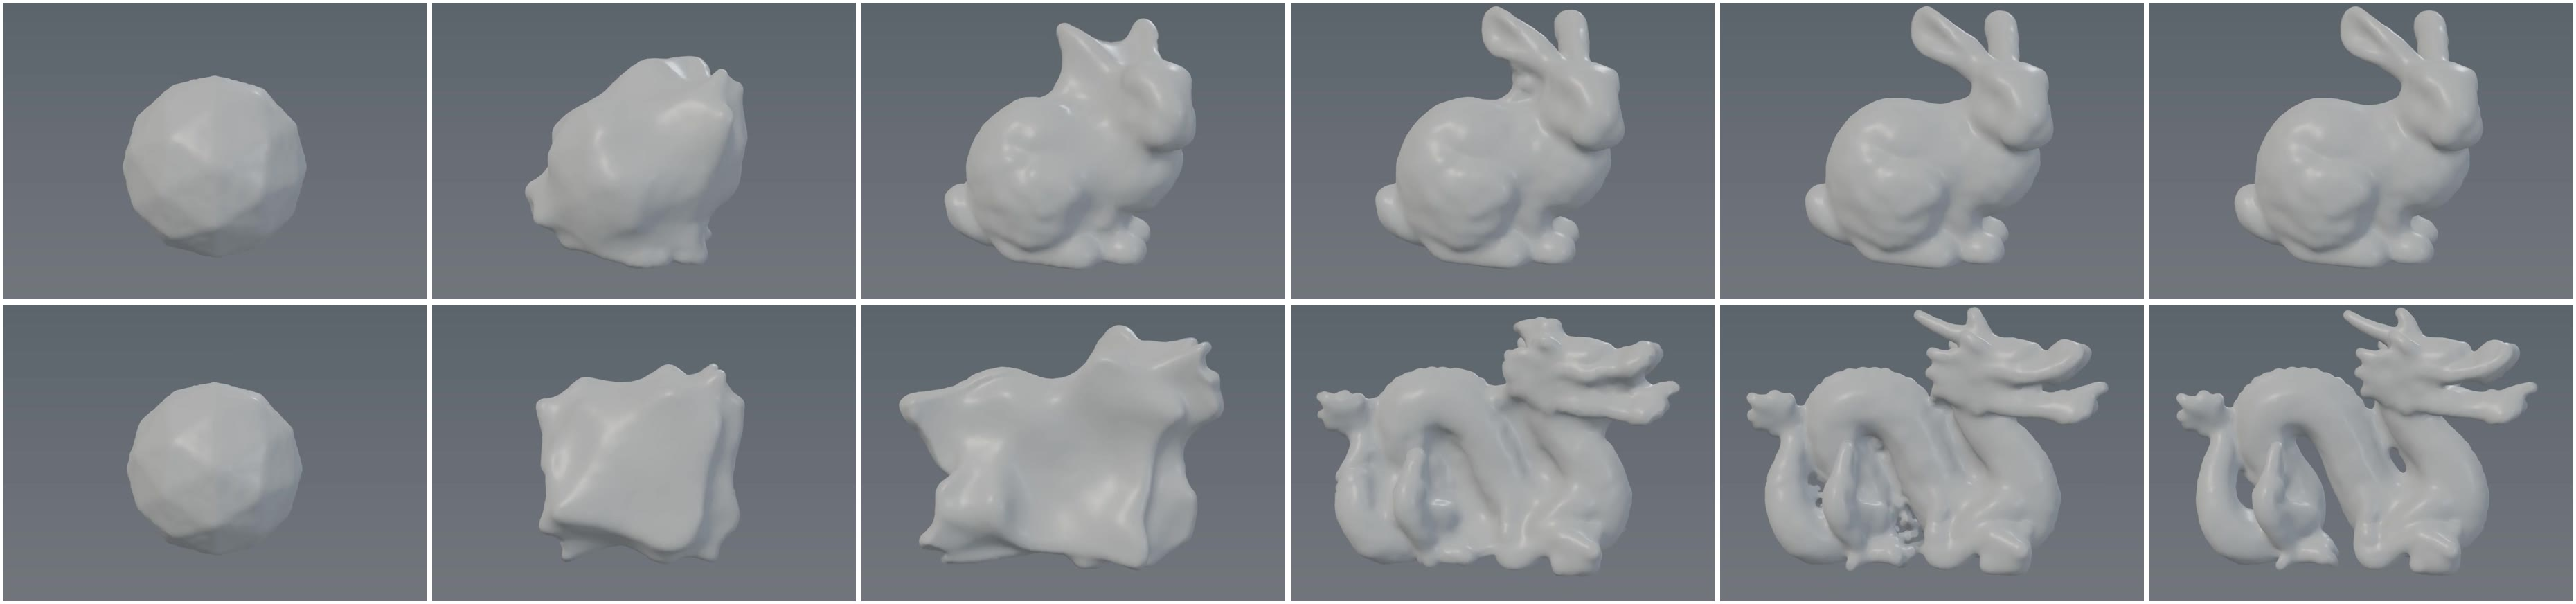
\includegraphics[width=\textwidth]{figs/ch4/fig_morph_sequence.jpg}
    \caption{Sphere to bunny and sphere to dragon at 300k particles. \textmd{The body rises as one piece and the features
    grow out of it in the first second; the dragon's narrowest gaps open last.}}
    \label{ch4:fig_morph}
\end{figure*}

\subsection{Sphere to Bunny and Dragon}
Figure~\ref{ch4:fig_morph} shows the bunny and the dragon. The body rises as one piece, and the features grow out of it
within the first second. Both the physics core and the render term do most of their drop in that time, the render term a
little behind because it reads a surface that is still arriving (Figure~\ref{ch4:fig_progress}). What follows is a long,
slow tail: most of the delivered frames, but only a small share of the particle movement, while both terms keep falling on
a logarithmic scale. The ends are close to what a perfect placement of the particles would give: the particle silhouette
lies just below the sampling floor and the chamfer distance below it, because the ends are more even than any random
sample. The bodies end at rest, and no run sheds a serious piece.

\begin{figure}[t]
    \centering
    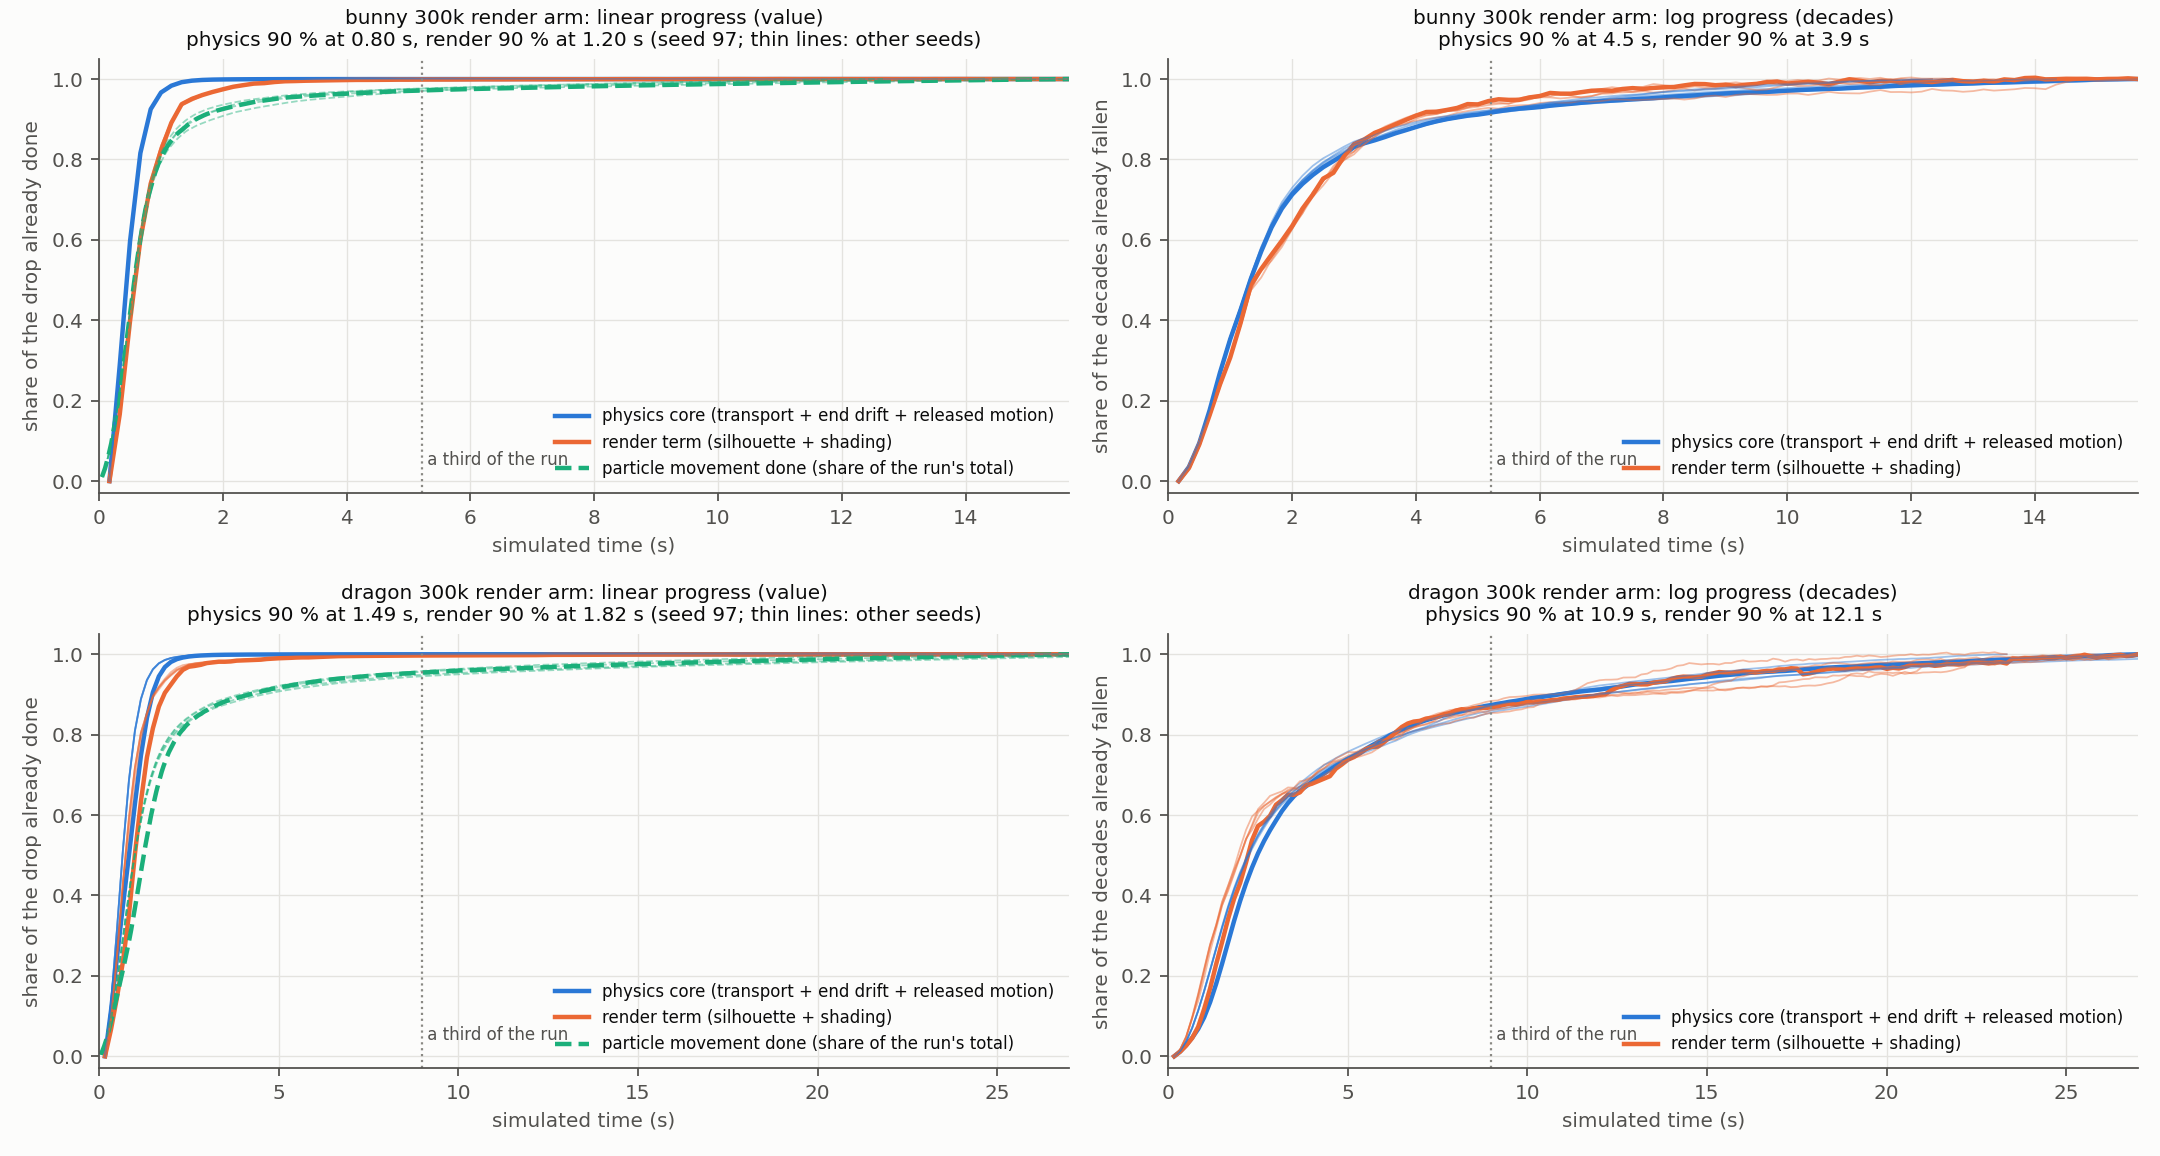
\includegraphics[width=\linewidth]{figs/ch4/fig_progress.png}
    \caption{How the objective falls over a 300k morph. \textmd{Physics and render terms both do most of their drop in the
    first second or two and keep falling on a logarithmic scale.}}
    \label{ch4:fig_progress}
\end{figure}

\subsection{What the Render Term Does}
\label{ch4:sec_render_effect}
We follow the render term through a run, against its twin, in three phases: the arrival, the time after it, and the end.

\textit{During the arrival, the render redirects material.} In the first second the full method's surface parts from its
twin's by far more than two runs of the same arm with different seeds part from each other; on the dragon the gap reaches
almost a pitch. The render carries only a small share of the surface's motion in that second, but that second holds most
of all the motion the morph makes. Figure~\ref{ch4:fig_rgv} shows where it acts: on the ears, the face and the feet,
mostly in agreement with the physics early on and more often in conflict later, where the projection removes the opposing
part.

\textit{After the arrival, it only polishes.} Once the body has arrived, the physics gradient has fallen by more than an
order of magnitude, and with it, by the rule of Section~\ref{ch4:sec_lambda}, the render weight and the step. The two arms'
surfaces return to a difference no larger than the seed-to-seed noise. What the render term still does is hold a sub-pitch
offset on silhouette rims and thin parts against the physics' own refit. A causal test shows this
(Figure~\ref{ch4:fig_switch}): switched off at 6\,s, the full method loses its lead within about a second; switched on at
6\,s, the twin builds it within a third of a second and ends level with the run that had the render throughout. Most of
what the render asks for lies below the MPM cell, and it is $u$, not $\delta\mathbf{F}_c$, that reaches it.

\textit{At the end, the gains are small but consistent.} Table~\ref{ch4:tab_d157} reads the end against the exact target
meshes, on views the loss never sees. At 300k every standard metric but one improves, in every mesh and in nearly every
pair of runs; the one exception is saturated. The improvement is real but small in absolute terms: the Boundary IoU error
goes from 0.068 to 0.054, near a perfect sample's 0.052. The gain is the same on views far from every training view, so it
is not specific to the pictures the loss sees; Table~\ref{ch4:tab_b1} gives it per mesh. At 40k the same metrics move in
the same direction, by about half as much on the boundary metrics and less elsewhere. The particle-level measures do not
see these gains: the particle silhouette, chamfer distance, thin coverage, centre of mass and rest stay within the twin's
range (Figure~\ref{ch4:fig_render_end}), because the binary particle silhouette resolves almost two pitches per pixel while
the render changes the exterior by fractions of a pitch (Figure~\ref{ch4:fig_iou}).

\begin{table}[t]
\centering
\footnotesize
\setlength{\tabcolsep}{4pt}
\caption{The full method against its $\lambda=0$ twin, read against the exact target mesh. \textmd{$r$ is the median share
of the twin's error the full method removes (for PSNR, the gain); $^\ast$ marks a metric that sees the render by the rule
fixed beforehand.}}
\label{ch4:tab_d157}
\begin{tabular}{lcccc}
\toprule
 & \multicolumn{2}{c}{300k (6 meshes, 22 pairs)} & \multicolumn{2}{c}{40k (19 meshes, 57 pairs)} \\
\cmidrule(lr){2-3}\cmidrule(lr){4-5}
metric & $r$ & pairs / meshes & $r$ & pairs / meshes \\
\midrule
\multicolumn{5}{l}{\textit{silhouettes, held-out views (1024\,px)}}\\
Boundary IoU (2\,\% of the diagonal) & $+16.3\,\%^\ast$ & 22 / 6 & $+7.1\,\%^\ast$ & 52 / 17 \\
boundary F-score (DAVIS, 12\,px)      & $+0.9\,\%$       & 12 / 3 & $+12.5\,\%$      & 31 / 11 \\
contour Chamfer                       & $+20.2\,\%^\ast$ & 21 / 6 & $+8.4\,\%^\ast$  & 54 / 18 \\
contour HD95                          & $+19.6\,\%^\ast$ & 21 / 6 & $+8.1\,\%^\ast$  & 50 / 18 \\
\multicolumn{5}{l}{\textit{3D, visible exterior}}\\
F-score at 0.5 pitch                  & $+36.4\,\%^\ast$ & 22 / 6 & $+8.0\,\%^\ast$  & 46 / 16 \\
F-score at 1 pitch                    & $+14.4\,\%^\ast$ & 22 / 6 & $+3.5\,\%$       & 39 / 15 \\
normal consistency                    & $+9.2\,\%^\ast$  & 21 / 6 & $+2.8\,\%$       & 42 / 15 \\
Chamfer-L1                            & $+12.9\,\%^\ast$ & 22 / 6 & $+4.3\,\%$       & 46 / 16 \\
\multicolumn{5}{l}{\textit{images, held-out views (512\,px)}}\\
shaded PSNR                           & $+0.73$\,dB$^\ast$ & 22 / 6 & $+0.30$\,dB$^\ast$ & 53 / 18 \\
shaded SSIM                           & $+10.7\,\%^\ast$ & 22 / 6 & $+3.0\,\%$       & 52 / 18 \\
shaded LPIPS                          & $+7.0\,\%^\ast$  & 22 / 6 & $+2.5\,\%$       & 47 / 17 \\
normal-map PSNR                       & $+0.96$\,dB$^\ast$ & 22 / 6 & $+0.36$\,dB$^\ast$ & 53 / 18 \\
normal-map SSIM                       & $+9.0\,\%^\ast$  & 22 / 6 & $+2.7\,\%$       & 51 / 17 \\
normal-map LPIPS                      & $+10.0\,\%^\ast$ & 22 / 6 & $+3.8\,\%$       & 51 / 17 \\
\midrule
\multicolumn{5}{l}{\textit{for comparison}}\\
particle silhouette IoU (128\,px)     & $+2.3\,\%$       & 14 / 4 & $+4.5\,\%$       & 48 / 19 \\
mask IoU against the raw mesh         & $+5.2\,\%$       & 22 / 6 & $-0.9\,\%$       & 19 / 5 \\
\bottomrule
\end{tabular}
\end{table}

\textit{Part of the render's lead on its own term is arrangement, not shape.} At the end of the 300k runs the full
method's render term lies below that of every uniform sample of the true mesh, which no body of the exact shape, sampled
uniformly, can do. What goes below that floor is an outer layer arranged more evenly, and hence an exterior smoother, than
any random sample; on the bunny at least two fifths of the full method's lead over its twin on the render term is of this
kind, and on the dragon at least a fifth. This is why we read shape only on the exact mesh and use the render terms' own
operators, as in Figures~\ref{ch4:fig_render_end} and~\ref{ch4:fig_switch}, only to locate the render's action.

In short, in the pipeline as it stands, the render term reshapes the arrival and polishes the end; after arrival it does
not decide anything that the physics objective leaves open. It also has a small cost: it deforms some bodies more, and the
ambient drag, which does not respect angular momentum, acts more on a body that moves more. Section~\ref{ch4:sec_costs}
takes up what the render could decide with more authority. Appendix~\ref{app:ch4_results} gives the measurements behind
this section.

\begin{figure*}[t]
    \centering
    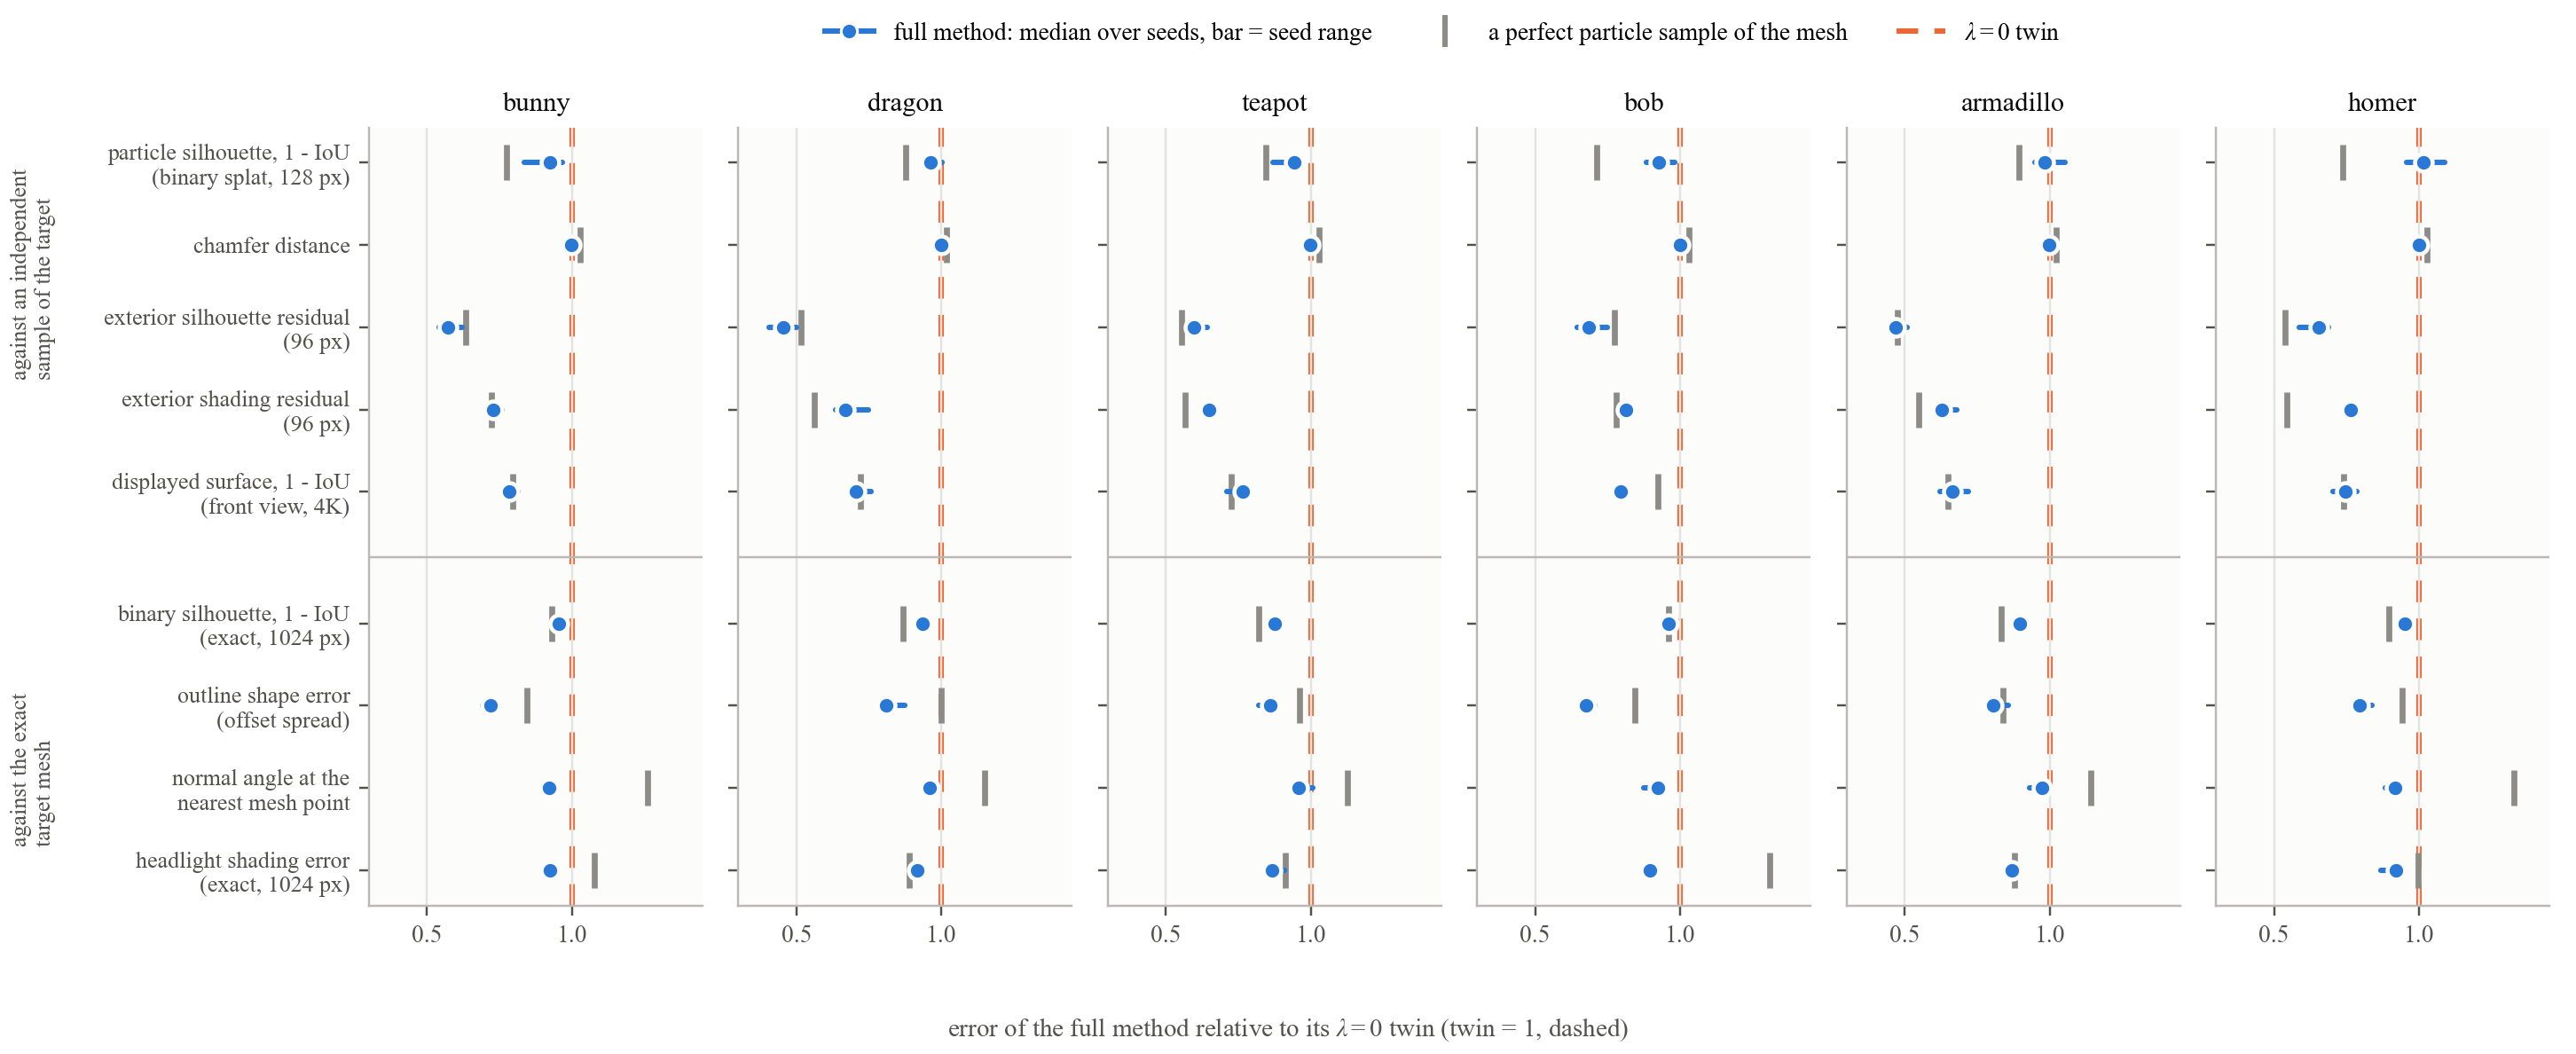
\includegraphics[width=\textwidth]{figs/ch4/fig_render_effect_end.png}
    \caption{The end of the run, full method against its $\lambda=0$ twin on six meshes. \textmd{The render terms' own
    residuals move the most, the exact-mesh readings less, and the particle IoU and chamfer hardly at all.}}
    \label{ch4:fig_render_end}
\end{figure*}

\begin{figure*}[t]
    \centering
    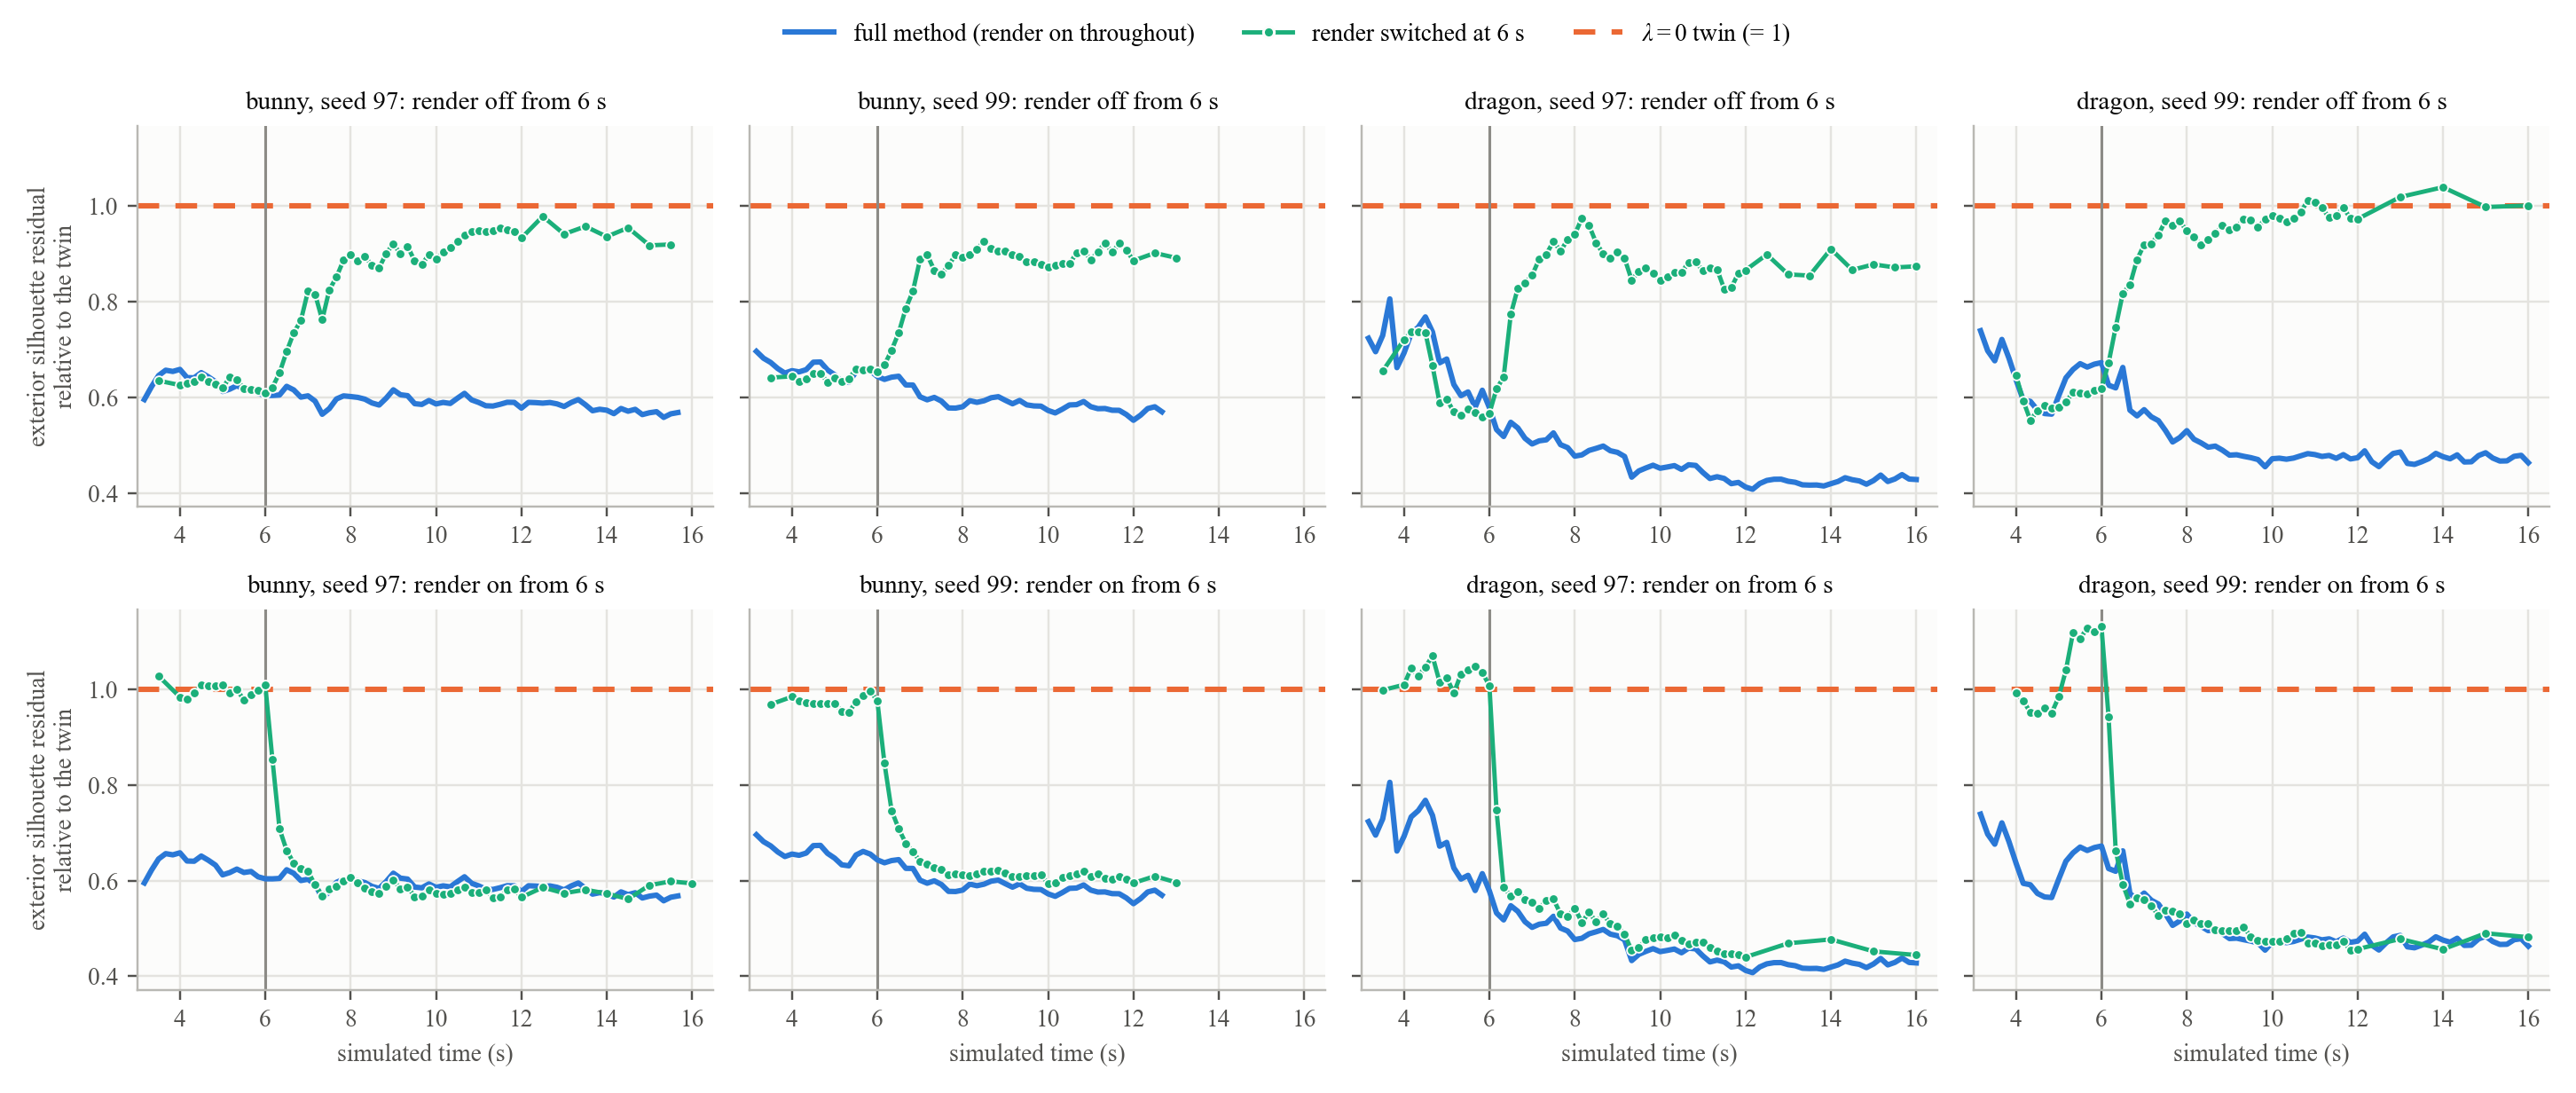
\includegraphics[width=\textwidth]{figs/ch4/fig_render_switch.png}
    \caption{The render term switched at 6\,s. \textmd{Switched off, the full method loses its lead within about a second;
    switched on, the twin builds it within a third of a second.}}
    \label{ch4:fig_switch}
\end{figure*}

\begin{figure*}[p]
    \centering
    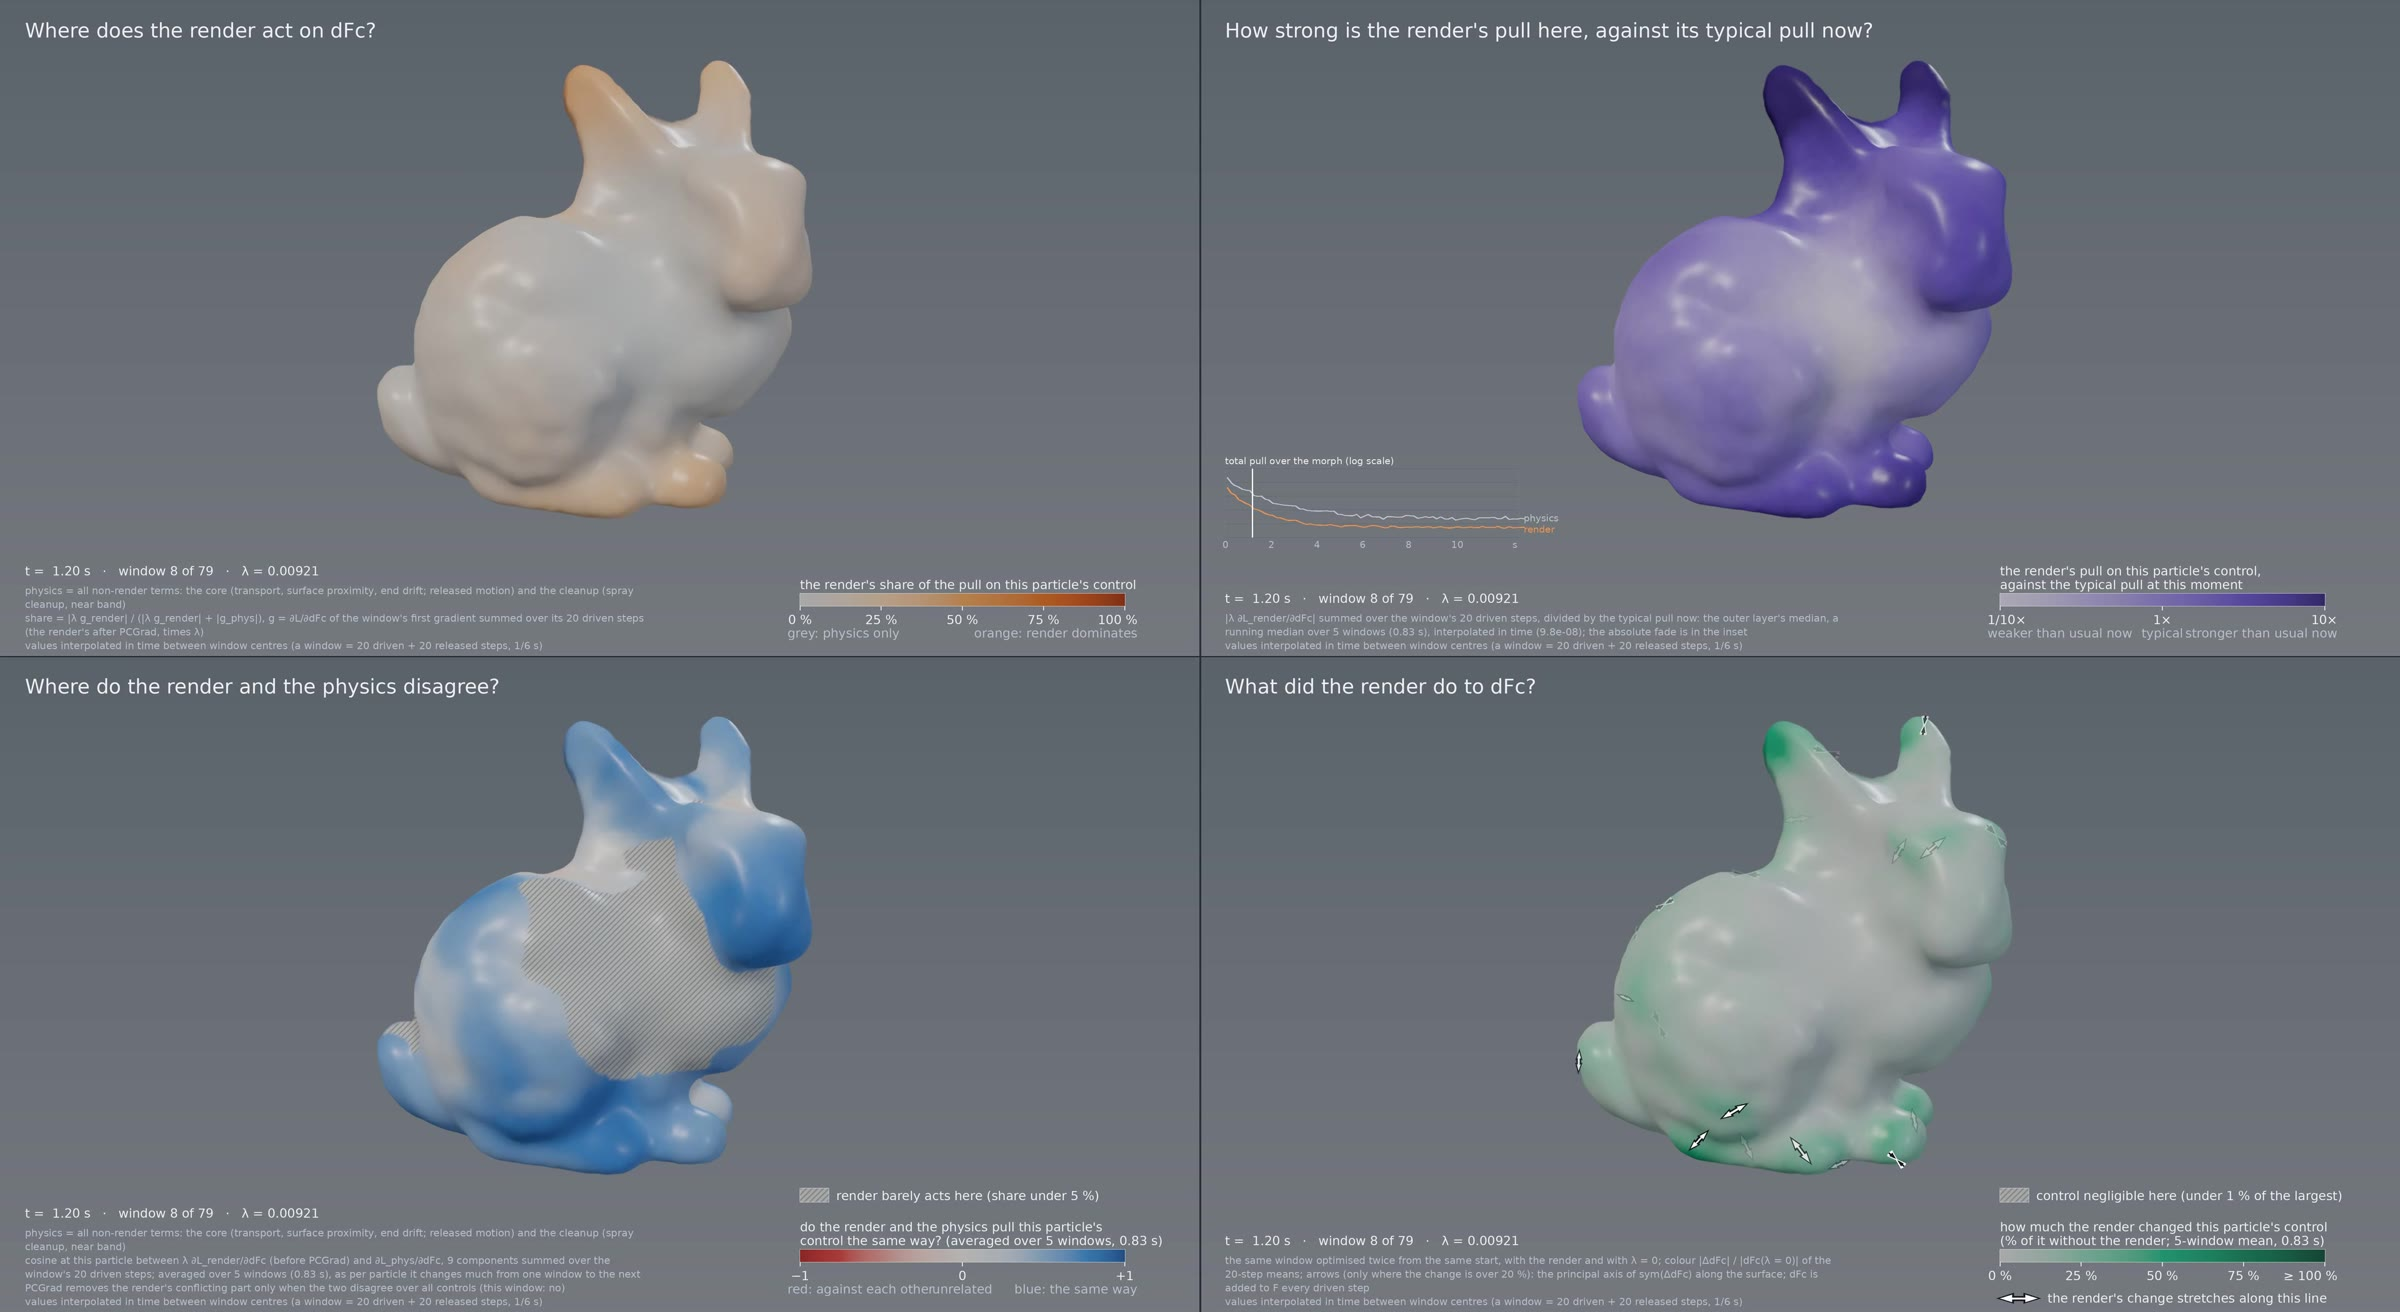
\includegraphics[width=\textwidth]{figs/ch4/fig_render_gradient_early.jpg}\\[4pt]
    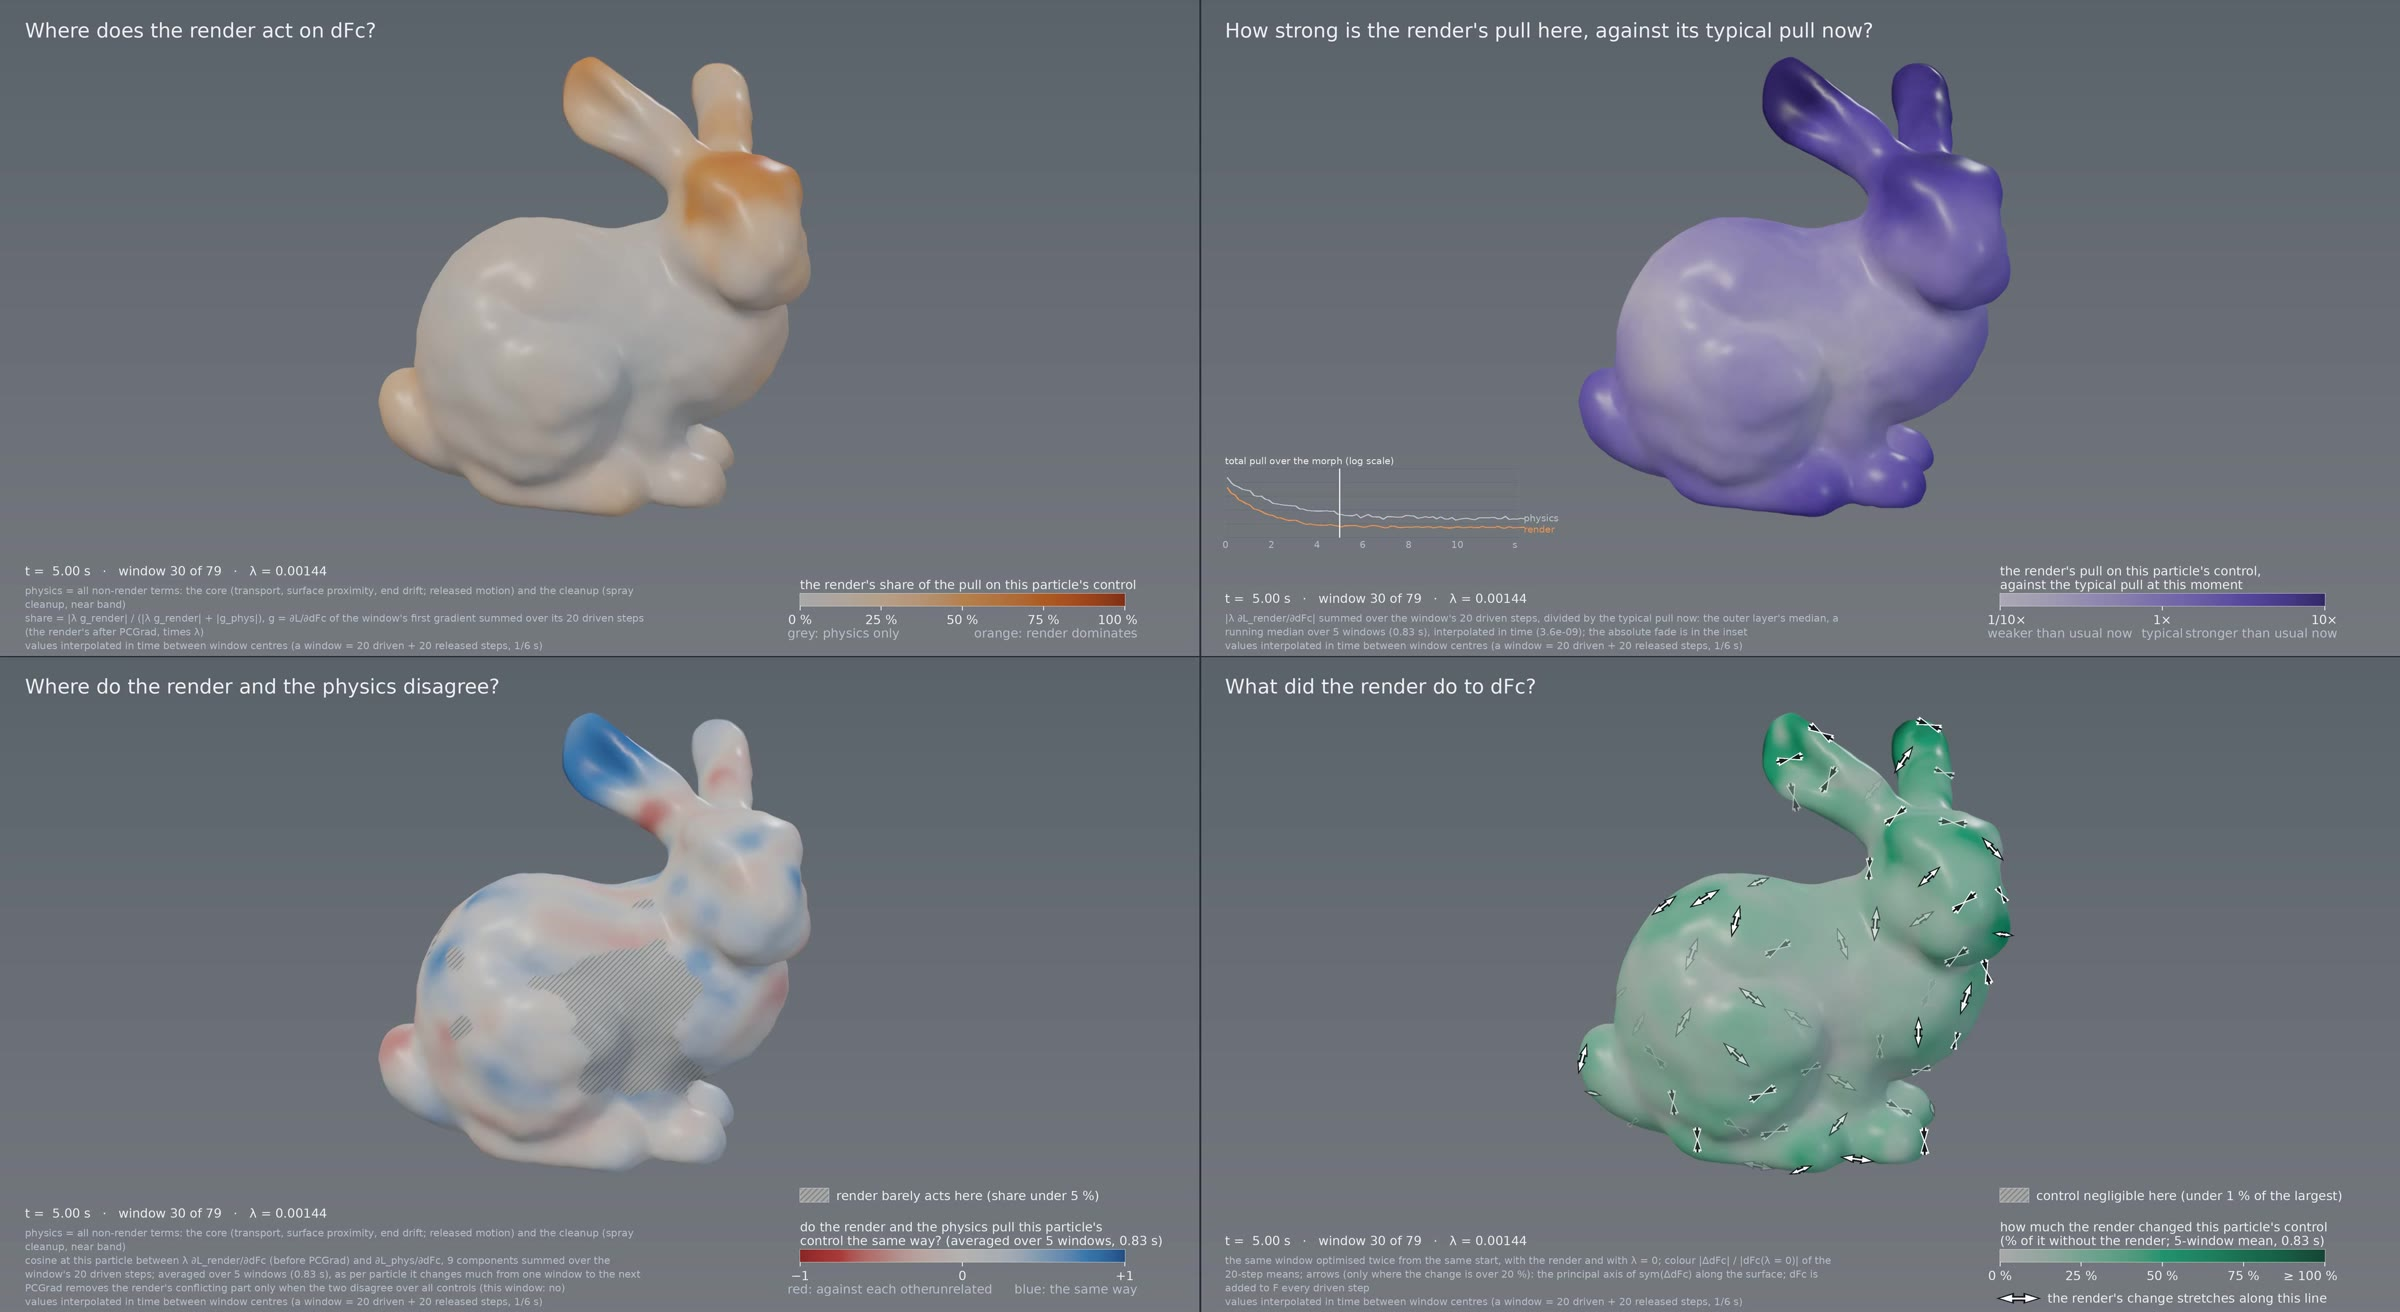
\includegraphics[width=\textwidth]{figs/ch4/fig_render_gradient_late.jpg}
    \caption{The render gradient on the deforming 300k bunny, early (top) and late (bottom). \textmd{Each block shows the
    render's share of each particle's pull, its strength, its agreement with the physics, and what it changed in
    $\delta\mathbf{F}_c$.}}
    \label{ch4:fig_rgv}
\end{figure*}

\subsection{The 40k Gallery}
\label{ch4:sec_gallery40}
On the 19-mesh gallery at $N=40{,}000$ the render acts in the same direction as at 300k, at about half the size: the
particle silhouette is ahead of the twin's on all but one mesh by a small margin, and against the exact meshes the outline
improves on all 19. One reading goes the other way: the silhouette area against the raw mesh is slightly worse, because the
exterior leans slightly outward. The lean comes from the silhouette term's asymmetric weighting of missing against excess
coverage, which at 40k, unlike at 300k, is not balanced by an inward pull; Appendix~\ref{app:ch4_gallery} gives the
measurement and the next test.

\subsection{A Gallery of 300k Morphs}
\label{ch4:sec_showcase}
To see the method beyond the six main targets, we ran it unchanged from a sphere to the 13 other gallery meshes and to the
Happy Buddha, a target of genus six, and between six pairs of shapes (Figure~\ref{ch4:fig_showcase}). Every run but one
reaches its target nearly as closely as the main six do, comes to rest, and sheds no serious piece. Topology changes as
the targets ask. From the teapot to bob, the teapot's handle closes within the first second and bob's ring opens later,
so the body ends with the target's single hole; from a sphere, the Happy Buddha's openings form. Where twins were run, the
render's lead has the same direction and size as on the main six.

Three examples show where the method still pays. On the letter C the run stops early while the body still flows, because
the stop rule reads the objective's progress, not rest. Between two shapes in different orientations, such as spot and the
cow, the transport carries the head over the back; yawing the source first makes the same morph direct and twice as fast.
And a less compact source such as the armadillo runs on a cell that is coarse relative to the body, and passes through
thin, perforated sheets on its way to homer.

\begin{figure*}[p]
    \centering
    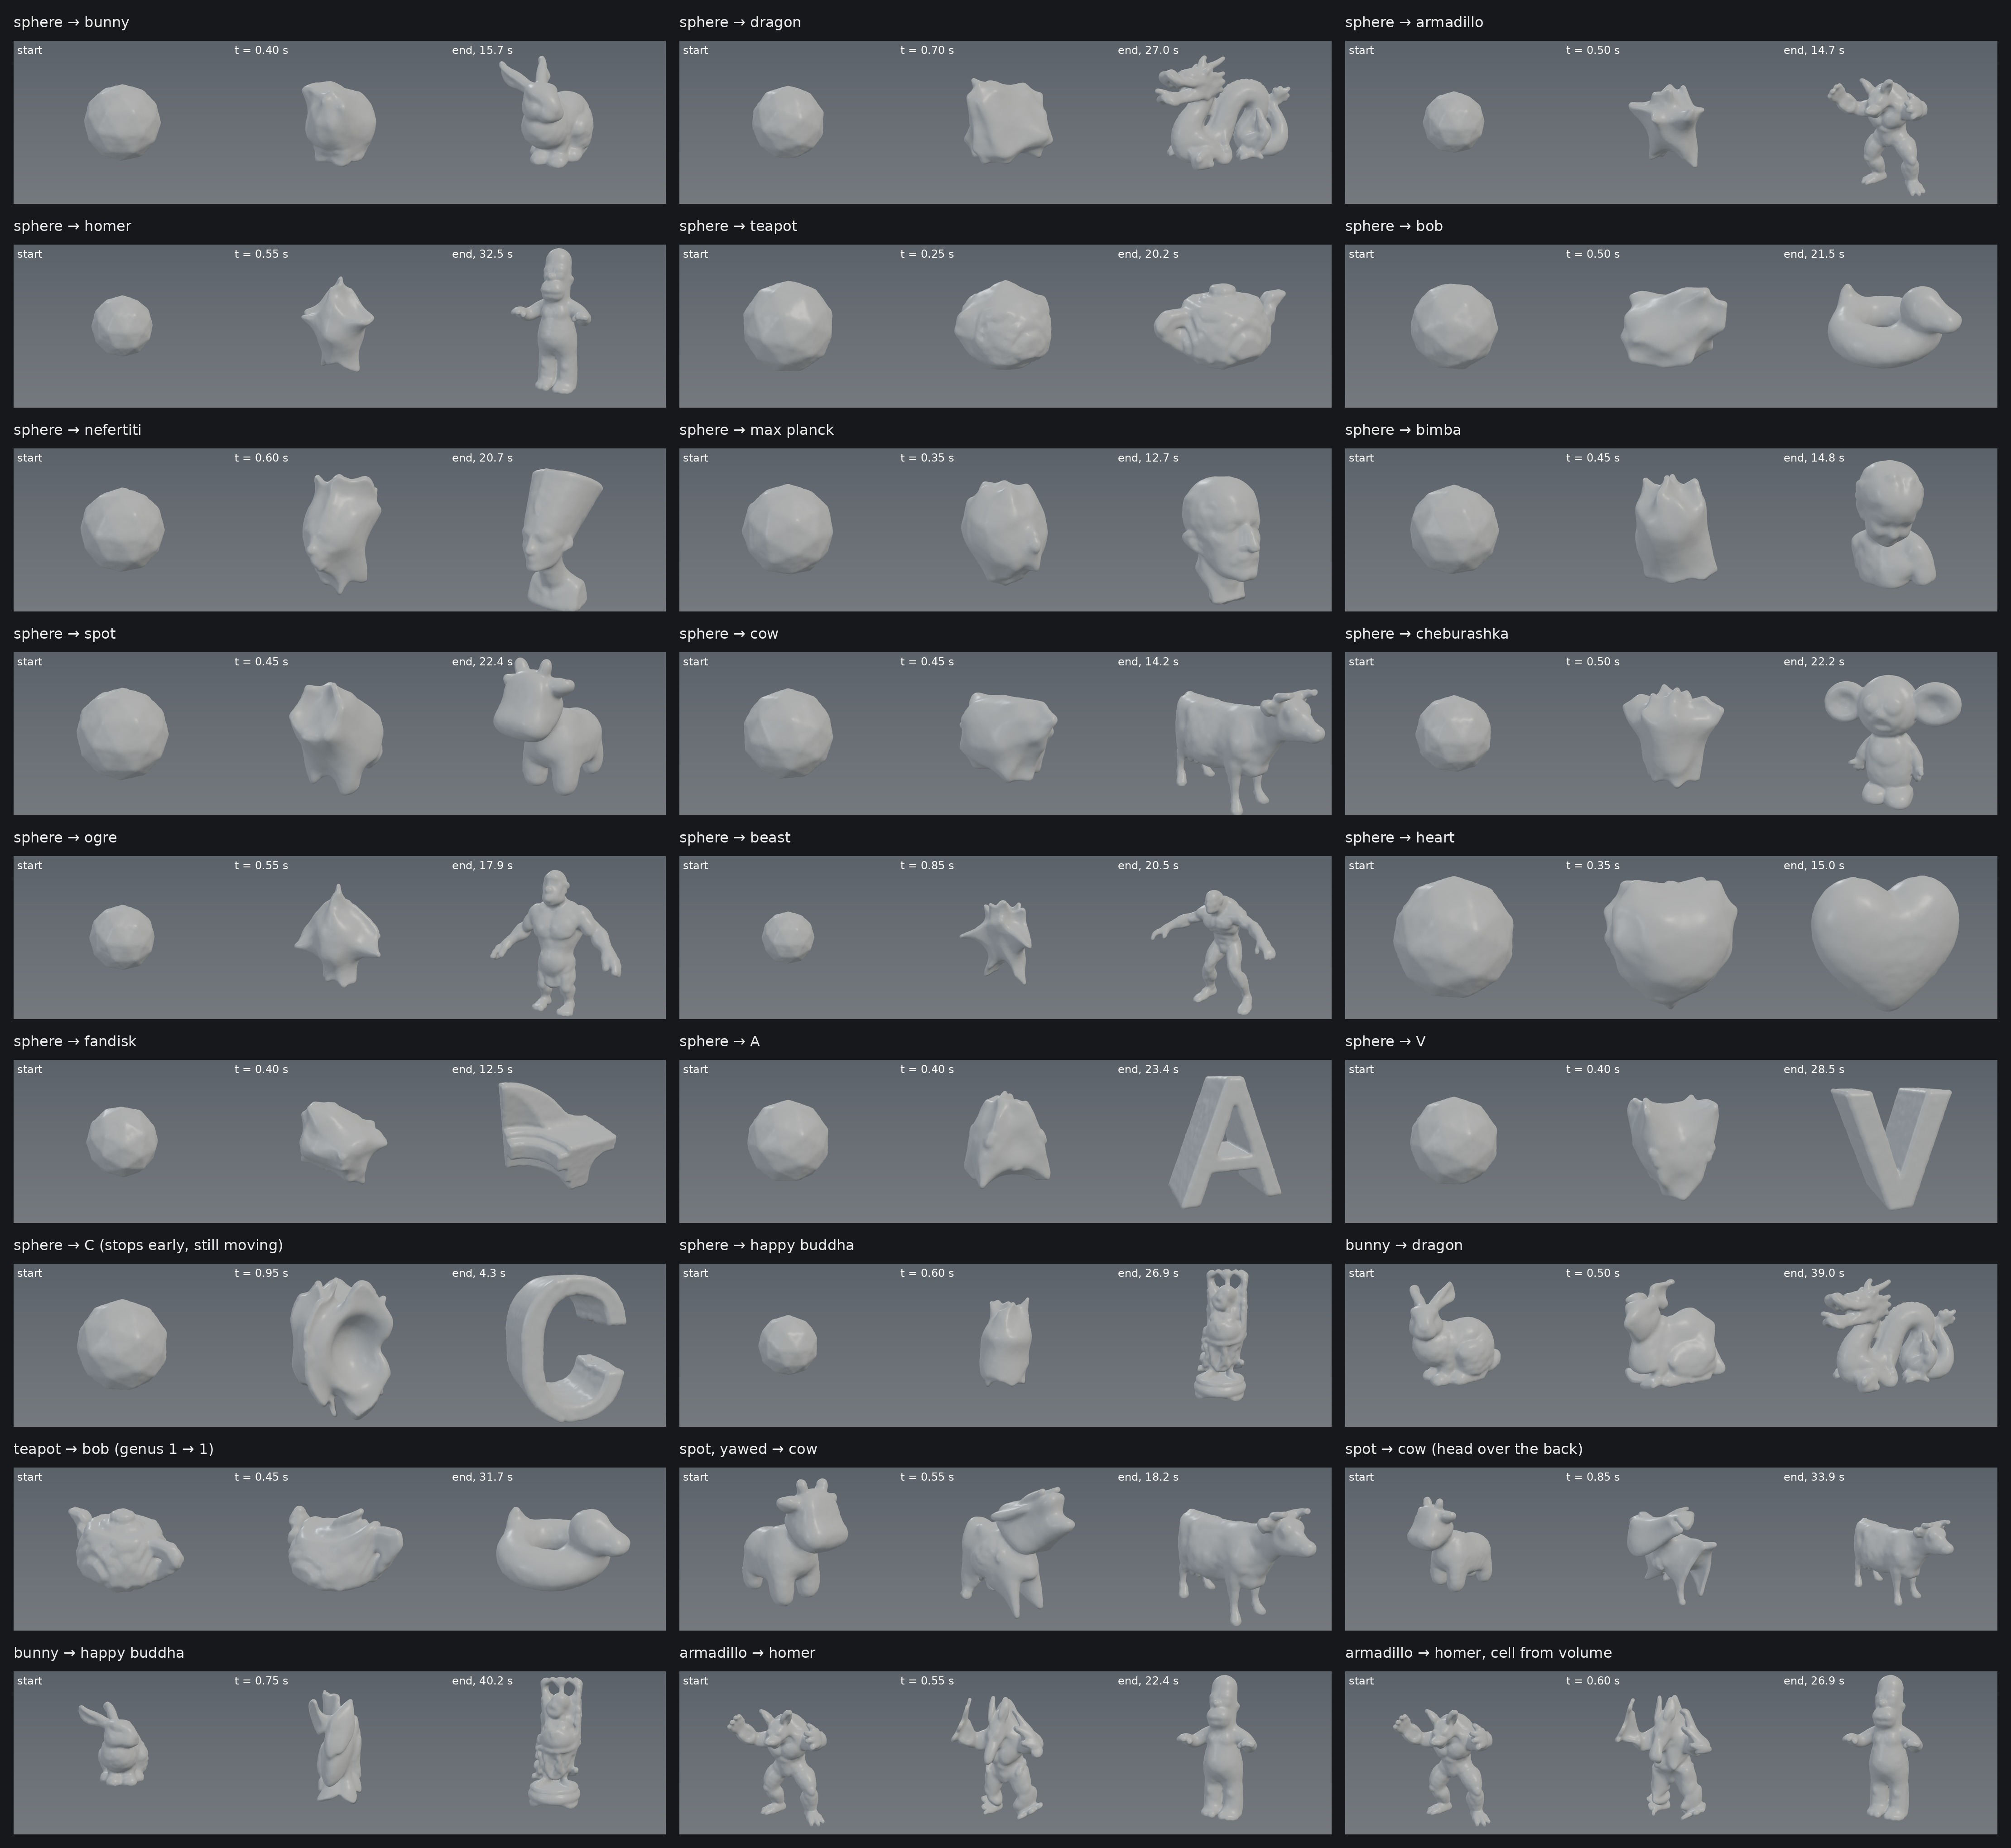
\includegraphics[width=\textwidth]{figs/ch4/fig_showcase_montage.jpg}
    \caption{Twenty-seven 300k morphs, each shown at its start, halfway and end. \textmd{The last panel uses an MPM cell
    set from the source's volume, an option outside the method, for comparison with the panel before it.}}
    \label{ch4:fig_showcase}
\end{figure*}

\subsection{Materials and External Forces}
Every material we tried reaches its target: a soft solid arrives more slowly, a stiff one faster but less at rest, and
the render term's lead holds in each. Under gravity, the single-body window stops early, because a falling body raises the
world-fixed objective. Through the scene path, with the target standing on the floor, the bunny and the dragon reach their
targets on every seed, stand upright at the target's height and keep their horizontal momentum. They do not come to rest:
each commit's assimilation makes part of the weight's sag rest shape and the controls raise it again. The next definition
assimilates only the controls' share of each window's deformation (Appendix~\ref{app:ch4_gravity}).

\subsection{Ablations}
\label{ch4:sec_ablation}
Switching off one part at a time at 300k (Table~\ref{ch4:tab_ablation}) gives three readings. First, $u$ is the main shape
lever: without it every surface measure is several times worse and the body never comes to rest, although the early
floating particles almost vanish, because $u$ is also their source. Second, reading the render on the exterior beats reading
it on the particle cloud on every measure of the surface, while the cloud read wins on the particle measures it optimizes;
each read wins on the representation it scores, and the exterior is the one a viewer sees. Third, the volume-conserving
body, the minimum spacing and the choices made against late motion each earn their place on what they address.

\subsection{Stress Control against Force Control}
\label{ch4:sec_force}
Classical physics-based shape control drives matter toward a target with external
forces~\citep{treuille2003keyframe,2004-FluidControlAdjointMethod,10.1145/1015706.1015743,chen2024eigenfluids,li2025flowmapadjoint}.
To test our choice, we replaced $\delta\mathbf{F}_c$ by an optimized external force per particle and step and kept
everything else. A plain force puts momentum in at every window, which the objective then has to pull back. Projecting the
force onto zero net force and torque removes that momentum exactly, but not the shape deficit: both force arms end with
several times the stress control's geometry energy and a worse surface, and they do not end more at rest. The stress
control gives exact momentum without a projection, and a better end than a momentum-free force reaches with the same
objective.

\subsection{Comparison with Other Methods}
\label{ch4:sec_comparison}
We compare with nine methods of five kinds, each run from the same sphere toward the same six targets and read by the same
probes: the F-control of Chapter~\ref{CH3_SHAPEMORPHING}~\citep{11088224}; the neural implicit morphs of Buonomo et
al.~\citep{buonomo2025vpnsm}, NISE~\citep{novello2023nise}, ISD~\citep{sang2025isd} and 4Deform~\citep{sang2025fourdeform};
as-rigid-as-possible interpolation~\citep{2000-ARAPShapeInterpolation}; optimal-transport displacement
interpolation~\citep{mccann1997convexity,bonneel2011displacement}; and render-only mesh optimization with Large
Steps~\citep{nicolet2021largesteps} and FlexiCubes~\citep{shen2023flexicubes}. Table~\ref{ch4:tab_methods} and
Appendix~\ref{app:ch4_comparison} give the full reading.

No method's silhouette lies above ours on any mesh, and the clearest separation is in the thin parts: ours leaves about as
many thin target points uncovered as a second sample of the mesh does, while every other method leaves at least half
again as many. What separates the methods most, however, is the way there. ISD fits the end but loses the body on the way;
Large Steps keeps one genus-zero surface and can never open a handle; FlexiCubes changes topology without control;
transport alone and the F-control of Chapter~\ref{CH3_SHAPEMORPHING} keep the mass but tear thin parts into clouds. Ours
stays one body with exact mass and a near-constant volume throughout and reaches every target, including those of higher
genus. Read on their own end meshes, the best mesh methods have sharper surfaces than our particle route, but a perfect
particle sample of the target trails them by a similar amount: that part of the gap is the cost of a particle body at this
resolution. The render-only mesh methods, ARAP, the F-control and NISE are faster than ours; ISD, the volume-preserving
morph and 4Deform are slower.

\subsection{Runtime}
\label{ch4:sec_runtime}
A 300k morph takes ten minutes to half an hour on one GPU (Table~\ref{ch4:tab_runtime}). The run length is set by the stop
rule, and most of it is the slow tail after arrival. That tail is not wasted: the end measures keep improving through its
first half and the body settles, and only its last tenth changes nothing measurable.

\subsection{Thrown and Dropped Bodies}
\label{ch4:sec_throw}
Two spheres are thrown toward each other, collide in the air while half-formed, part, and each becomes a bunny that lands
and tumbles (Figure~\ref{ch4:fig_throw}). The scene uses the multi-body definitions of Appendix~\ref{ch4:sec_scene} and a
stiffer material, with the plastic assimilation off so that the controls hold each body's shape against the impacts. In
the delivered run the bodies meet when the morph is a little under half done, separate cleanly, land, spring off the floor
and tumble, and each ends close to its target in its own frame, with momentum kept through every phase. A single body can
fall as well: a sphere released high above the floor becomes a bunny on the way down, lands, bounces, and tips forward
onto its head, which the body-frame objective allows.

\begin{figure*}[tbp]
    \centering
    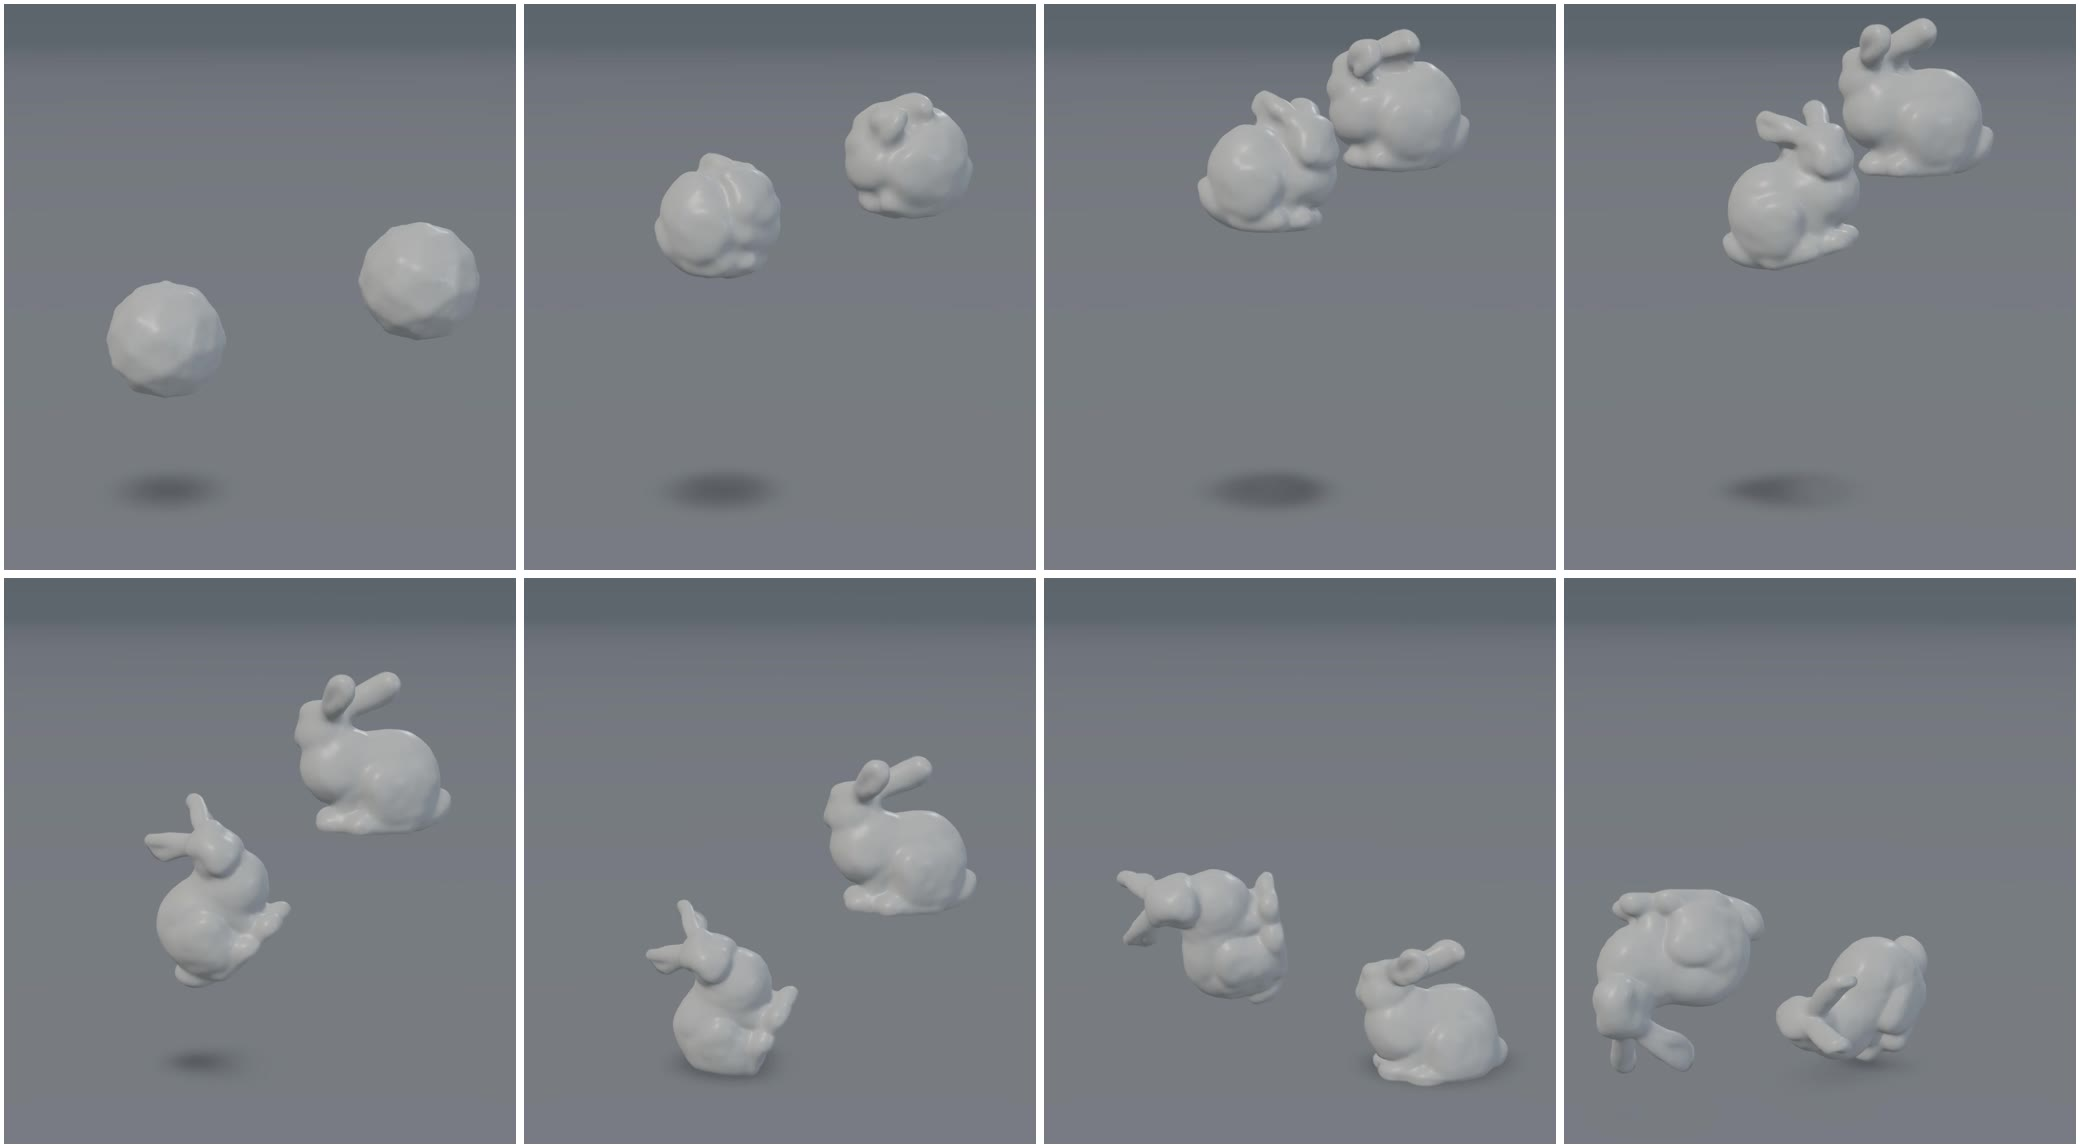
\includegraphics[width=\textwidth]{figs/ch4/fig_throw_scene.jpg}
    \caption{Two thrown bodies, each becoming a bunny. \textmd{Each body has its own grid field and its own objective in its
    own frame, so they part cleanly, fly, land and tumble.}}
    \label{ch4:fig_throw}
\end{figure*}

% ============================================================================
\section{Measured Costs and Next Steps}
\label{ch4:sec_costs}
% ============================================================================

\textbf{Giving the render its authority after arrival.} The results above locate the render's limit precisely. Every
physics term reads only the set of particle positions, so the physics objective cannot tell which material ends where,
nor relief finer than the 3D target resolves; these are exactly the things only a picture can decide. Yet after arrival
the render weight follows the vanishing physics gradient, so the render has no authority left when there is something
only it could decide. Our ongoing experiments keep that authority by holding the render weight at its first calibrated
value. With a colour term held this way, the body routes its coloured material to the layout of the target pictures, which
the physics objective cannot see, and recovers most of the layout's error. With the full render weight held, lettering that
exists only in the target pictures is carved into the particles of a plaque, to more than half of the relief a sample of the
lettered mesh carries. Both runs currently end with the body still moving, because a held weight does not vanish once the
body has arrived. The open question is a weight definition that keeps the render's authority where it has something to
decide and lets the body come to rest; the definition under test follows the render term's own excess over a measured
floor.

\textbf{Transient floaters.} The early arrival leaves a few particles apart from the body, mostly relief standing half a
pitch outside the displayed surface. None persists, and on the display surface none forms a separate piece. Their main
source is $u$; a link that keeps each layer step near its neighbour removed most of them but moved the centre of mass, and
the next form makes that link symmetric, as the minimum spacing is.

\textbf{Narrow gaps.} The cubic kernel averages the grid velocity over about two cells, so a gap of the target narrower
than that cannot open until late and tears into beads when it does. An MPM cell that follows $N$ opens the teapot's handle
and sharpens the boundaries, but leaves most of the dragon's loops closed, fills the early surface with holes and more
than doubles the dragon's cost. A finer cell is therefore an option of the pipeline, to be chosen after the same comparison
on more meshes.

\textbf{Angular momentum and the drag.} The ambient drag damps the particle momentum but not APIC's affine part. A drag that
damps the whole APIC momentum cut the largest angular momentum several-fold on a test body and kept shape and rest.

\textbf{A long, slow tail.} Most of the delivered frames come after the arrival. A target that moves along the transport's
displacement interpolation over the body's elastic period spreads the deformation in time, lowers the kinetic peak and the
early loose particles, keeps the render's lead, and ends at rest, but its end trails the fixed target's slightly on a few
meshes; the next measurement tells a shorter refit from under-supplied extremities.

\textbf{A target given only by pictures.} When the 3D target is the visual hull of the training silhouettes and only the
render terms see the true mesh, the full method sharpens the held-out outline but does not carve the concavities that only
the pictures hold. The information is in the pictures, but only a smooth change of the whole surface lowers the loss; a
multiview shape-from-shading descent finds the concave regions in place, and the next step carves them from a hull that
contains the object at the render's resolution.

% ============================================================================
\section{Chapter Summary}
\label{ch4:sec_summary}
% ============================================================================

This chapter presented a render-guided morphing pipeline built on the differentiable MLS-MPM of
Chapter~\ref{CH3_SHAPEMORPHING}. The body is a volume-conserving solid driven by a capped stress increment and a rigid-free
offset of its outer layer. It is optimized in settled windows, each scored after the controls are released, by a
transport energy, settling and cleanup terms, and the silhouette and shading of its own exterior surface.

The morph keeps exact mass and, up to the ambient drag, momentum; it ends at rest, opens handles a sphere does not have,
runs unchanged on a wide range of targets and shape pairs, and takes part in contact and gravity with other bodies. Against
nine other methods, no method's silhouette lies above ours on any mesh, and only ours keeps thin parts at the sampling
floor. The render term's role is measured as well: it redirects material while the body arrives, then only polishes rims
because its weight follows the vanishing physics gradient, and it leaves the end consistently but slightly closer to the
exact target, with part of its lead on its own term coming from a smoother arrangement rather than a different shape. The
next step is to give the render its authority after arrival, where it can decide what the physics objective cannot see.

% Dissertation build: end of the chapter-only stretch set at its start.
\setlength{\emergencystretch}{0pt}
